\documentclass[a4paper,11pt]{report}
\usepackage[utf8]{inputenc}
\usepackage[OT1]{fontenc}
\usepackage[italian]{babel}
\usepackage{fancyhdr}
\usepackage{indentfirst}
\usepackage{amsmath}
\usepackage{amsfonts}
\usepackage{graphicx}
\usepackage{caption}
\usepackage{subcaption}
\usepackage{vicent}
\usepackage{float}

\newenvironment{system}{\left\lbrace \begin{aligned}}{\end{aligned}\right.}

\title{\bfseries{\Huge{Laboratorio di Fisica Computazionale}}}
\author{\cursiveshape {Luca Cassia - [MAT. 728341]}}

\date{Spring 2012}

\pagestyle{fancy}\addtolength{\headwidth}{20pt}
\renewcommand{\chaptermark}[1]{\markboth{\thechapter.\ #1}{}}
\renewcommand{\sectionmark}[1]{\markright{\thesection \ #1}{}}
\cfoot{}

\rhead[\fancyplain{}{\bfseries\leftmark}]{\fancyplain{}{\bfseries\thepage}}
\lhead[\fancyplain{}{\bfseries\thepage}]{\fancyplain{}{\bfseries\rightmark}}

\begin{document}
\maketitle
\tableofcontents

\chapter{\huge Integrazione Numerica}

\textit{In analisi numerica, l'integrazione numerica consiste in un insieme di metodi che stimano il valore di un integrale definito, senza dover calcolare la primitiva della funzione integranda. In questa sezione si illustrano alcuni dei principali metodi deterministici e non deterministici.}

\section{Newton-Cotes}
Le regole di quadratura di Newton-Cotes sono formule che consistono nel valutare l'integrando in punti equispaziati dell'intervallo di integrazione.

Si assume che il valore di una funzione $f:[a,b]\subset\mathbb{R}\rightarrow\mathbb{R}$ sia noto nei punti $x_i$, per $i=0,...,n$ tali che $$x_i=a+\left(\frac{b-a}{n}\right)i$$
La formula di Newton-Cotes di grado $n$ si ottiene interpolando $f$ nei punti $x_i$ con i polinomi della base di Lagrange~\cite{uno}, e integrando la polinomiale risultante, $L(x)$, nell'intervallo $[a,b]$.
$$ \int_a^b f(x) \,dx \approx \int_a^b L(x)\,dx = \int_a^b \bigl( \sum_{i=0}^n f(x_i)\, \ell_i(x) \bigr) \, dx = \sum_{i=0}^n f(x_i) \underbrace{\int_a^b \ell_i(x)\, dx}_{w_i} $$
dove gli $\ell_i(x)$ sono i polinomi di Lagrange così definiti
$$\ell_i(x):= \prod_{\begin{smallmatrix}0\le j\le n\\ j\neq i\end{smallmatrix}} \frac{x-x_j}{x_i-x_j}$$$$\ell_i(x_j)=\delta_{ij}$$
La formula di Newton-Cotes assume così la semplice forma di media dei valori $f(x_i)$ pesati sui coefficienti $w_i$ (indipendenti da $f$)
$$\int_a^b f(x) \,dx \approx \sum_{i=0}^n w_i\, f(x_i)$$
Si domostra che l'errore dell'interpolazione di $f$ con un polinomio è
$$E(x)=\frac{1}{(n+1)!}f^{(n+1)}(\xi(x))\prod_{i=0}^n(x-x_i)$$
per un certo $\xi\in[a,b]$ dipendente da $x$. Non avendo tuttavia alcuna informazione su come individuare il punto $\xi$ in genere si effettua solo una stima del limite superiore sull'errore $E(x)$ per $\xi$ tale che $f(\xi) = \underset{x\in[a,b]}{\max}f(x)$.

Al primo ordine dell'approssimazione Newton-Cotes la formula si riduce al cosidetto metodo dei ``trapezi'':
$$\int_a^b f(x) \,dx=\frac{b-a}{2}\left[ f(a)+f(b)\right] + \underbrace{\frac{1}{2}\int_a^b f''(\xi(x))(x-a)(x-b)}_{E_1}$$
mentre al secondo ordine non è altro che la regola di Simpson:
\begin{multline*}
\int_a^b f(x) \,dx=\frac{b-a}{3}\left[f(a)+4f(\frac{a+b}{2})+f(b)\right] +\\ + \underbrace{\frac{1}{6}\int_a^b f'''(\xi(x))(x-a)(x-\frac{a+b}{2})(x-b)}_{E_2}
\end{multline*}

\section{Quadrature Gaussiane}
La regola di quadratura Gaussiana a $n$-punti è un metodo di integrazione numerica costruito in modo tale da fornire un risultato esatto per polinomi di grado inferiore a $2n$, attraverso una scelta appropriata di punti $x_i$ e pesi $w_i$, per $i=1,...,n$. Sul dominio di integrazione convenzionale $[-1,1]$ la regola è così formulata
$$\int_{-1}^1 f(x)\,dx \approx \sum_{i=1}^n w_i f(x_i)$$
L'accuratezza del risultato è tanto più grande quanto meglio $f$ è approssimata da un polinomio. Se tuttavia la funzione integranda può essere scritta come $f(x)=W(x)g(x)$, dove $g(x)$ è approssimativamente polinomiale e $W(x)$ è nota, allora esistono $w'_i$ tali che
$$\int_{-1}^1 f(x)\,dx = \int_{-1}^1 W(x) g(x)\,dx \approx \sum_{i=1}^n w_i' g(x_i)$$
$W(x)$ viene detta funzione peso, mentre i punti $x_i$ sono le radici di un polinomio appartenente alla classe dei polinomi ortogonali.

Nel caso considerato $W(x)=1$ ed i polinomi associati sono i polinomi ortogonali di Legendre $P_n(x)$~\cite{uno}. Il peso $i$-esimo associato al nodo Gaussiano $x_i$ è dato da
$$ w_i = \frac{2}{\left( 1-x_i^2 \right) [P'_n(x_i)]^2} \,\!$$
Analogamente alle regole di Newton-Cotes, l'errore teorico del metodo della quadratura Gaussiana è
$$E(x)=\frac{1}{n!}f^{(n)}(\xi(x))\prod_{i=1}^n(x-x_i)$$
che può tuttavia essere ridotto a
$$E(x)=\frac{1}{(2n)!}f^{(2n)}(\xi(x))\prod_{i=1}^n(x-x_i)^2$$
semplicemente considerando due volte ogni punto di interpolazione $x_i$.

Infine, se si vuole calcolare l'integrale su $[a,b]$ invece che sull'intervallo $[-1,1]$, si deve effettuare il cambio di variabile
$$\int_a^b f(x)\,dx = \frac{b-a}{2} \int_{-1}^1 f\left(\frac{b-a}{2}x + \frac{a+b}{2}\right)\,dx $$
ed applicando il metodo di Gauss si ottiene
$$\int_a^b f(x)\,dx \approx \frac{b-a}{2} \sum_{i=1}^n w_i f\left(\frac{b-a}{2}x_i + \frac{a+b}{2}\right)$$
I nodi ed i pesi per il polinomio di Legendre di quinto grado sono riportati in tabella:\\
\begin{center}
\scalebox{1.5}{
\begin{tabular}{c c}
\hline
$x_i$ & $w_i$ \\
\hline\hline
$0$ & $\frac{128}{255}$ \\
$\pm\tfrac13\sqrt{5-2\sqrt{10/7}}$ & $\tfrac{322+13\sqrt{70}}{900}$ \\
$\pm\tfrac13\sqrt{5+2\sqrt{10/7}}$ & $\tfrac{322-13\sqrt{70}}{900}$ \\
\end{tabular}
}
\end{center}

\subsection{Integrazione Composta}
Una tecnica utile a migliorare la precisione del calcolo dell'integrale numerico consiste nello spezzare l'intervallo d'integrazione in $n$ sottointervalli
$$\int_a^b f(x)dx=\sum_{i=0}^{n-1}\int_{\frac{b-a}{n}i}^{\frac{b-a}{n}(i+1)}f(x)dx$$
Dopodiché si applica uno dei metodi di quadratura numerica descritto ad ogni intervallino ed infine si somma ad ottenere il risutato richiesto.

\section{Monte Carlo}
L'integrazione Monte Carlo~\cite{sei}, a differenza dei metodi di quadratura precedentemente descritti, fa uso di sampling casuali e per questo motivo rientra nella categoria dei metodi non deterministici.

Nella sua versione più semplice l'algoritmo consiste nell'estrarre uniformemente punti dalla regione di integrazione per stimare l'integrale ed il relativo errore. Si supponga che il sample sia costituito da $N$ punti $x_1,...,x_N$ appartenenti alla regione di integrazione di misura $V$, allora la stima dell'integrale è data da
$$ I \approx E_N \equiv V\frac{1}{N} \sum_{i=1}^N f(x_i) = V \langle f \rangle $$
Poichè $\{x_i\}$ è una sequenza di punti equidistribuiti in $V$, si può dimostrare che $ I = \lim_{N \to \infty} E_N $.
Tenendo presente che la varianza della funzione integranda è
$$ \mathrm{Var}(f)\equiv\sigma_N^2 = \frac{1}{N-1} \sum_{i=1}^N (f(x_i) - \langle f \rangle)^2$$
la varianza di $E_N$ è quindi
$$ \mathrm{Var}(E_N) =  \frac{V^2}{N^2} \sum_{i=1}^N \mathrm{Var}(f)  =V^2 \frac{\mathrm{Var}(f)}{N} = V^2\frac{\sigma_N^2}{N}$$
Dal momento che le considerazioni appena fatte rimangono valide anche nel caso multidimensionale, quello che si deduce è che l'errore sulla stima dell'integrale scala come $1/\sqrt{N}$, indipendentemente dal numero di dimensioni.

\subsection{Campionamento di Importanza}
Dal punto di vista metematico, il campionamento di importanza corrisponde al cambio di variabile
$$\int f(x) \,dx = \int\frac{f(x)}{p(x)}\,p(x)\,dx = \int\frac{f(x)}{p(x)}\,dP(x)$$
con $$p(x)=\frac{\partial^d}{\partial x_1...\partial x_d}\,P(x)$$
Se si restringe $p(x)$ ad essere una funzione a valori non negativi normalizzata all'unità, allora si può interpretare $p(x)$ come una densità di probabilità. Se poi si ha a disposizione un generatore di numeri casuali corrispondente alla distribuzione $P(x)$ si può anche stimare l'integrale da un sample $x_1,...,x_N$ di numeri casuali distribuiti secondo $P(x)$
$$E_N = \frac{1}{N}\sum_{n=1}^N\frac{f(x_n)}{p(x_n)}$$
L'errore statistico dell'integrazione Monte Carlo è dato da $\sigma(f/p)/\sqrt N$.

Il campionamento di importanza è efficace se si sceglie $p(x)$ tale che approssimi bene $|f(x)|$ e tale che si sia capaci di generare numeri casuali con distribuzione di probabilità $P(x)$.

\section{Esempi}
Si dimostrano ora i metodi descritti nei paragrafi precedenti applicandoli al calcolo di alcuni integrali particolari. Le funzioni integrande scelte sono:
\begin{figure}[H]
\centering
\begin{tabular}{lccl}
funzione & & & primitiva\\\\
$\log(1+x)$ & & & $-x + \log(1 + x) + x \log(1 + x)$\\\\
$x^9 - x^7 + 3$ & & & $\frac{x^{10}}{10} - \frac{x^8}{8} + 3x$
\end{tabular}
\end{figure}
Tutti gli integrali sono calcolati tenendo fisso l'intervallo d'integrazione $I=[1,2]$ e variando il numero di suddivisioni per ogni metodo. Conoscendo inoltre l'espressione analitica delle primitive delle due funzioni integrande è possibile calcolare i risultati esatti ed usare questi ultimi per confrontare l'errore del risultato numerico con l'errore previsto. Si sono calcolati analiticamente dunque alcuni valori utili alla stima di tale errore:
\\

\begin{figure}[H]
\centering
\begin{tabular}{ccc}
$f$ & $\max(f^{(1)})$ & $\max(f^{(4)})$\\
\hline
$\log(1+x)$ & $0.5$ & $-0.0740742$\\
$x^9 - x^7 + 3$ & $1856$ & $90048$
\end{tabular}
\end{figure}

In seguito si indicheranno con $E(f)$ l'errore stimato analiticamente e con $\Delta(f)$ l'errore calcolato numericamente.

\subsection{Newton-Cotes 1}

\begin{figure}[H]
 \begin{subfigure}[b]{0.5\textwidth}
  \centering
  \includegraphics[width=\textwidth]{integral1a}
  \caption{Log}
 \end{subfigure}
 \begin{subfigure}[b]{0.5\textwidth}
  \centering
  \includegraphics[width=\textwidth]{integral1b}
  \caption{Pol}
 \end{subfigure}
\caption{Confronto errore NC1 calcolato numericamente (rosso) e previsto analiticamente (blu).}
\label{fig:integral1}
\end{figure}

\begin{figure}[H]
 \begin{subtable}[b]{0.5\textwidth}
  \centering\small
\begin{tabular}{lll}
\hline
$n$ & $\Delta(Log)$ & $E(Log)$\\
\hline
10 & 1.388645e-04 & 4.166667e-04\\
20 & 3.472070e-05 & 1.041667e-04\\
40 & 8.680460e-06 & 2.604167e-05\\
80 & 2.170133e-06 & 6.510417e-06\\
160 & 5.425343e-07 & 1.627604e-06\\
320 & 1.356337e-07 & 4.069010e-07\\
640 & 3.390842e-08 & 1.017253e-07\\
1280 & 8.477104e-09 & 2.543132e-08\\
2560 & 2.119278e-09 & 6.357829e-09\\
5120 & 5.298190e-10 & 1.589457e-09\\
10240 & 1.324540e-10 & 3.973643e-10\\
20480 & 3.311029e-11 & 9.934107e-11\\
40960 & 8.277934e-12 & 2.483527e-11\\
81920 & 2.073119e-12 & 6.208817e-12\\
\end{tabular}
 \end{subtable}
 \begin{subtable}[b]{0.5\textwidth}
  \centering\small
\begin{tabular}{lll}
\hline
$n$ & $\Delta(Pol)$ & $E(Pol)$\\
\hline
10 & 1.541035e+00 & 1.546667e+00\\
20 & 3.860018e-01 & 3.866667e-01\\
40 & 9.654698e-02 & 9.666667e-02\\
80 & 2.413966e-02 & 2.416667e-02\\
160 & 6.035096e-03 & 6.041667e-03\\
320 & 1.508785e-03 & 1.510417e-03\\
640 & 3.771970e-04 & 3.776042e-04\\
1280 & 9.429930e-05 & 9.440104e-05\\
2560 & 2.357483e-05 & 2.360026e-05\\
5120 & 5.893707e-06 & 5.900065e-06\\
10240 & 1.473427e-06 & 1.475016e-06\\
20480 & 3.683568e-07 & 3.687541e-07\\
40960 & 9.208927e-08 & 9.218852e-08\\
81920 & 2.302198e-08 & 2.304713e-08\\
\end{tabular}
 \end{subtable}
\end{figure}

Come previsto, l'errore calcolato segue l'andamento ricavato analiticamente pur rimanendo sempre al di sotto di quest'ultimo. $E(f)$ infatti è solo il limite superiore per l'errore $\Delta(f).$ Nel caso della polinomiale inoltre i due errori risultano particolarmente vicini.

\subsection{Newton-Cotes 2}

\begin{figure}[H]
 \begin{subfigure}[b]{0.5\textwidth}
  \centering
  \includegraphics[width=\textwidth]{integral2a}
  \caption{Log}
 \end{subfigure}
 \begin{subfigure}[b]{0.5\textwidth}
  \centering
  \includegraphics[width=\textwidth]{integral2b}
  \caption{Pol}
 \end{subfigure}
\caption{Confronto errore NC2 calcolato numericamente (rosso) e previsto analiticamente (blu).}
\label{fig:integral2}
\end{figure}

\begin{figure}[H]
 \begin{subtable}[b]{0.5\textwidth}
  \centering\small
\begin{tabular}{lll}
\hline
$n$ & $\Delta(Log)$ & $E(Log)$\\
\hline
10 & 6.101824e-09 & 8.230467e-08\\
20 & 3.816787e-10 & 5.144042e-09\\
40 & 2.386025e-11 & 3.215026e-10\\
80 & 1.491696e-12 & 2.009391e-11\\
160 & 9.325873e-14 & 1.255870e-12\\
320 & 6.328271e-15 & 7.849185e-14\\
640 & 5.551115e-16 & 4.905740e-15\\
1280 & 1.443290e-15 & 3.066088e-16\\
2560 & 1.110223e-15 & 1.916305e-17\\
5120 & 2.442491e-15 & 1.197691e-18\\
10240 & 1.443290e-15 & 7.485566e-20\\
20480 & 4.440892e-15 & 4.678479e-21\\
40960 & 9.992007e-16 & 2.924049e-22\\
81920 & 3.996803e-15 & 1.827531e-23\\
\end{tabular}
 \end{subtable}
 \begin{subtable}[b]{0.5\textwidth}
  \centering\small
\begin{tabular}{lll}
\hline
$n$ & $\Delta(Pol)$ & $E(Pol)$\\
\hline
10 & 9.908609e-04 & 1.000533e-01\\
20 & 6.203492e-05 & 6.253333e-03\\
40 & 3.878841e-06 & 3.908333e-04\\
80 & 2.424535e-07 & 2.442708e-05\\
160 & 1.515373e-08 & 1.526693e-06\\
320 & 9.471108e-10 & 9.541829e-08\\
640 & 5.920242e-11 & 5.963643e-09\\
1280 & 3.666401e-12 & 3.727277e-10\\
2560 & 1.421085e-13 & 2.329548e-11\\
5120 & 1.278977e-13 & 1.455968e-12\\
10240 & 2.842171e-14 & 9.099798e-14\\
20480 & 4.263256e-14 & 5.687374e-15\\
40960 & 7.105427e-14 & 3.554608e-16\\
81920 & 5.684342e-14 & 2.221630e-17\\
\end{tabular}
 \end{subtable}
\end{figure}

L'errore per il metodo NC2 si comporta come previsto finchè non raggiunge valori dell'ordine di grandezza di $10^{-14}$ per i quali la precisione finita del calcolatore limita la precisione del calcolo introducendo del rumore nei dati.

\subsection{Quadratura Gaussiana 5}

\begin{figure}[H]
 \begin{subtable}[b]{0.5\textwidth}
  \centering
\begin{tabular}{lll}
\hline
$n$ & $\Delta(Log)$\\
\hline
10 & 2.220446e-16\\
20 & 2.220446e-16\\
40 & 1.110223e-16\\
80 & 0.000000e+00\\
160 & 5.551115e-16\\
320 & 1.110223e-15\\
640 & 2.220446e-16\\
1280 & 1.332268e-15\\
2560 & 1.110223e-15\\
5120 & 2.664535e-15\\
10240 & 1.110223e-16\\
20480 & 4.440892e-15\\
40960 & 9.992007e-16\\
81920 & 3.996803e-15\\
\end{tabular}
 \end{subtable}
 \begin{subtable}[b]{0.5\textwidth}
  \centering
\begin{tabular}{lll}
\hline
$n$ & $\Delta(Pol)$\\
\hline
10 & 0.000000e+00\\
20 & 0.000000e+00\\
40 & 0.000000e+00\\
80 & 0.000000e+00\\
160 & 0.000000e+00\\
320 & 1.421085e-14\\
640 & 0.000000e+00\\
1280 & 1.421085e-14\\
2560 & 1.136868e-13\\
5120 & 1.136868e-13\\
10240 & 1.421085e-14\\
20480 & 4.263256e-14\\
40960 & 8.526513e-14\\
81920 & 5.684342e-14\\
\end{tabular}
 \end{subtable}
\end{figure}

Nel caso della quadratura gaussiana di quinto grado l'errore decresce molto più rapidamente, tanto che già con poce decine di intervalli il risultato può essere considerato sufficientemente preciso. Dopo di chè i dati sono troppo disturbati dal rumore per poterne ricavare un andamento funzionale. Si nota inoltre che per il polinomio l'errore è esattamente zero come previsto dalla teoria.
\\

\subsection{Monte Carlo}
\begin{figure}[H]
\begin{subfigure}[b]{0.5\textwidth}
\centering
\includegraphics[width=\textwidth]{integral4a}
\caption{Log}
\end{subfigure}
\begin{subfigure}[b]{0.5\textwidth}
\centering
\includegraphics[width=\textwidth]{integral4b}
\caption{Pol}
\end{subfigure}
\caption{In rosso l'errore MC in funzione del numero di elementi del sample ed in blu la funzione $1/\sqrt{N}$.}
\label{fig:integral4}
\end{figure}

Per analizzare il comportamento dell'errore dei metodi Molte Carlo si studia ora il caso di un integrale di volume bidimensionale. Il dominio di integrazione è l'insieme $\Omega = \{(x,y)\in \mathbb{R}\,|\, x^2+y^2<1\,\wedge\, x,y>0\}$ mentre la funzione integranda non è altro che la costante $1$. Si utilizza la convenzionale funzione di misura $d\mu=dxdy$. La misura di $\Omega$ allora è facile da calcolare essendo l'area di un quarto di circonferenza goniometrica: $$\int_\Omega d\mu = \tfrac{\pi}{4}$$
La distribuzione dell'errore MC in funzione del numero di elementi del sample deve verificare la relazione $\sigma_{MC}\simeq 1/\sqrt N$.
\\

In figura \ref{fig:pi} sono rappresentati in scala bilogaritmica i dati ottenuti da $50000$ esecuzioni dell'algoritmo implementante il metodo Monte Carlo. In ascissa sono riportati i numeri delle dimensioni del sample mentre sulle ordinate sono ripotati i rispettivi errori.\\
Come previsto, la distribuzione ottenuta risulta centrata sulla curva $1/\sqrt{N}$ che è proprio l'errore stimato teoricamente.
\begin{figure}[H]
\centering
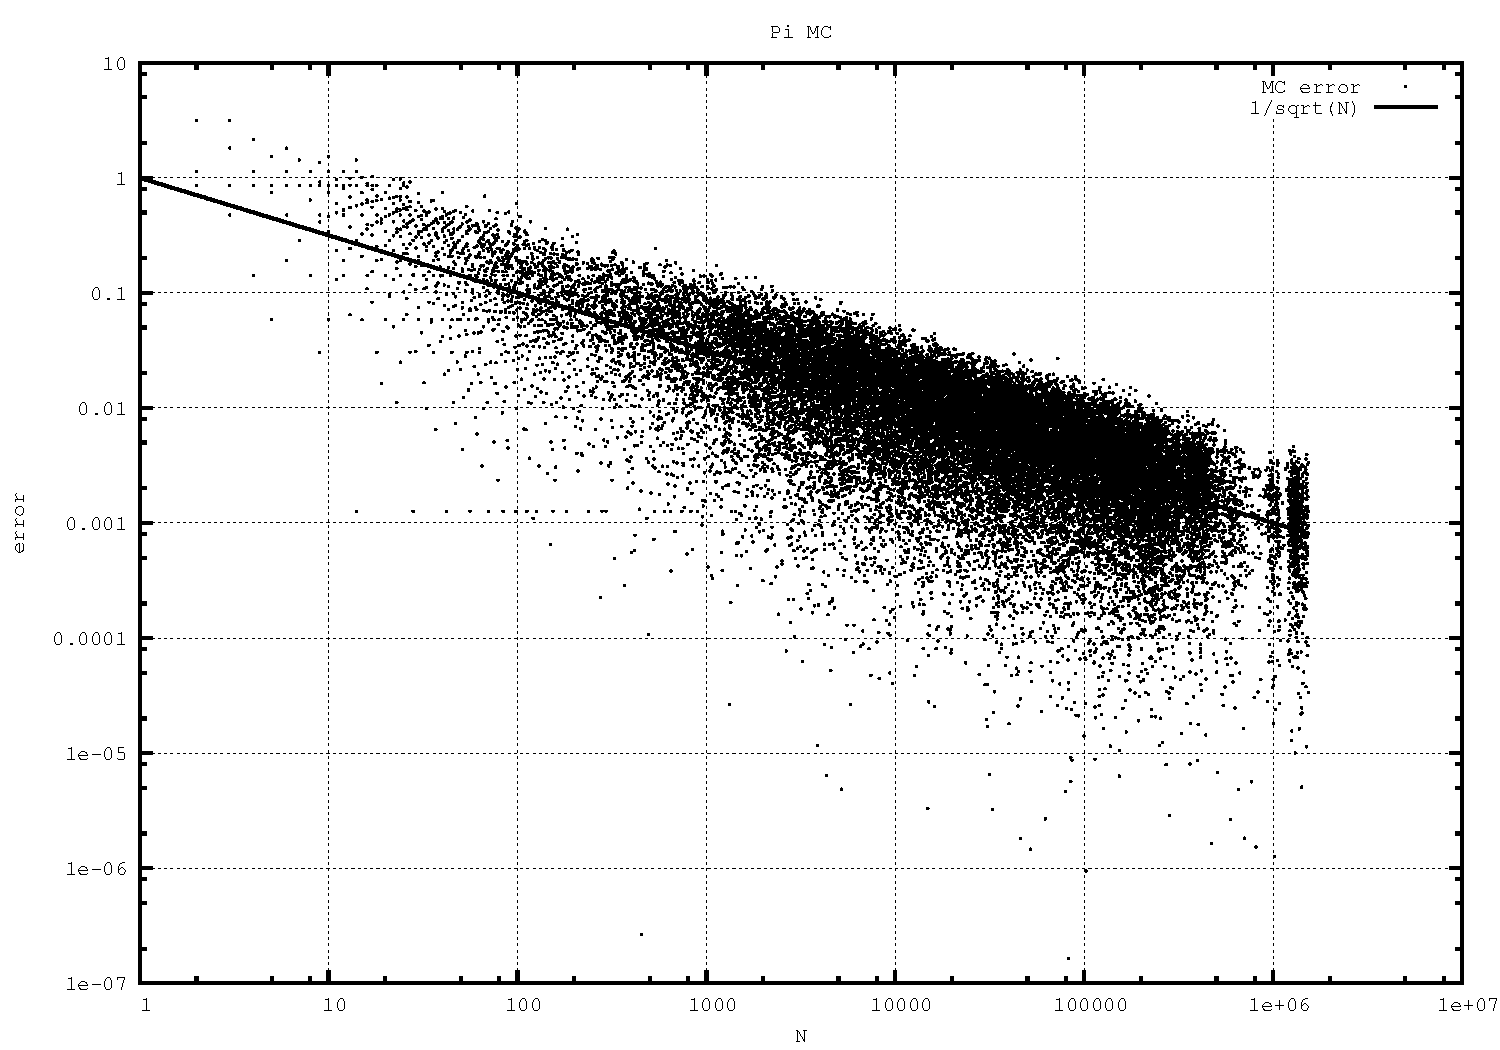
\includegraphics[width=\textwidth]{pi}
\caption{Distribuzione dell'errore MC in funzione del numero di elementi del sample. La linea continua rappresenta la funzione $1/\sqrt{N}$.}
\label{fig:pi}
\end{figure}


\chapter{\huge Algoritmo Metropolis}

\textit{Il Metropolis è l'algoritmo più influenziale fra quelli appartenenti alla classe dei metodi Monte Carlo. Supportato da un'ampia teoria sulle catene di Markov~\cite{due}, questo algoritmo costituisce uno strumento fondamentale per la scienza della computazione.}

\textit{In questa sezione si propone di sviluppare un algoritmo Metropolis per simulare un oscillatore armonico quantistico e confrontare i risultati numerici con la teoria.}
\\

Il metodo Metropolis~\cite{quattro} nasce dalla necessità pratica di dover generare numeri casuali distribuiti con una densità di probabilità $p(x_1,...,x_d)$, che non necessariamente fattorizza. Sia il vettore $\phi = (x_1,...,x_d)$ uno stato dell'ensemble, che vogliamo generare. L'algoritmo consiste nel partire da uno stato iniziale $\phi_0$, e sostituire iterativamente uno stato vecchio con uno nuovo, in maniera tale da ottenere la distribuzione corretta nel limite di un gran numero di iterazioni. La distribuzione che viene raggiunta all'equilibrio è indipendente dallo stato iniziale $\phi_0$. Una volta che tale distribuzione è stata raggiunta, l'applicazione ripetuta dell'algoritmo mantiene il sistema all'interno dello stesso ensemble. In altre parole, la distribuzione desiderata costituisce l'unico punto fisso dell'algoritmo.

Due condizioni importanti devono essere soddisfate per poter applicare il Metropolis: Ergodicità e bilancio dettagliato. La condizione di bilancio dettagliato afferma che le probabilità di transizione $W(\phi_1\rightarrow\phi_2)$ e $W(\phi_2\rightarrow\phi_1)$ rispettano l'equazione $$p(\phi_1)W(\phi_1\rightarrow\phi_2) = p(\phi_2)W(\phi_2\rightarrow\phi_1)$$
L'ergodicità invece richiede che ogni stato dell'ensemble possa essere raggiunto in un numero finito di steps.

Dato uno stato iniziale $\phi_1$, un'iterazione dell'algoritmo consiste delle seguenti istruzioni:
\begin{itemize}
    \item generare con distribuzione piatta un nuovo candidato $\phi'$ nell'intorno di $\phi$ di raggio $\delta$
    \item calcolare $\Delta S = -\log(p(\phi')/p(\phi_1))$
    \item se $\Delta S < 0$ impostare il nuovo stato $\phi_2=\phi'$
    \item se $\Delta S > 0$ accettare il nuovo candidato con probabilità $p(\phi')/p(\phi_1)$, altrimenti mantenere $\phi_1$
    \item passare all'iterazione successiva
\end{itemize}
L'algoritmo Metropolis tuttavia presenta alcuni svantaggi, tra i quali il fatto che quando si raggiunge la distribuzione d'equilibrio, gli stati successivi sono in genere molto correlati. Se si vuole ottenere un unbiased sample di stati $\phi_i$ si possono quindi trascurare un numero $\tau_d$ di stati prima di passare a quello successivo. Il numero di steps $\tau_d$ viene denominato tempo di decorrelazione ed è dell'ordine di $\xi^2$, dove $\xi$ è una tipica distanza di correlazione del sistema. Ciò è dovuto al fatto che il Metropolis aggiorna gli stati localmente in maniera casuale. L'agoritmo consiste quindi nell'eseguire un random walk attraverso lo spazio delle configurazioni, il che richiede $\xi^2$ passaggi per effettuare uno spostamento di una distanza $\xi$ in una certa direzione.

\section{Oscillatore Armonico}
Il sistema è costituito da una particella che si muove in uno spazio unidimensionale e in un reticolo temporale finito di passo $a$ e lunghezza $N$ con condizioni di periodicità al contorno. Le variabili del sistema sono quindi le coordinate $x_t$ della particella ai vari istanti di tempo $t$, con la condizione $x_N \equiv x_0$. La particella interagisce inoltre con un potenziale armonico della forma $$V(x) = \frac{m}{2}\omega^2 x^2$$

In meccanica quantistica la stima di un osservabile può essere estratta dalle funzioni di correlazione del sistema~\cite{otto}.
Si calcola quindi il correlatore delle variabili $l$-esima e $k$-esima $\langle x_lx_k\rangle$, definito dalla formula
$$\langle x_lx_k\rangle=\frac{\int Dx\ x_lx_ke^{-S_E}}{\int Dx\ e^{-S_E}}$$
Calcolare il correlatore significa calcolare un \textit{path integral}~\cite{sette} usando come ampiezza di probabilità il fattore $e^{-S_E}$. Il ruolo dell'algoritmo Metropolis è dunque quello di generare configurazioni del sistema con distribuzione di ampiezza di probabilità $e^{-S_E}$.
\\

Dopo aver ottenuto una stima per il correlatore delle variabili $x_l$ e $x_k$ per ogni combinazione di $(l,k)$, si ricavano infine i valori di $\Delta E=(\tilde{E}_1-\tilde{E}_0)$ e dell'elemento di matrice $W=\langle\tilde{E}_0|\hat{x}|\tilde{E}_1\rangle$ invertendo la relazione
\begin{center}
\small
$\langle x_l x_k\rangle = 2|\langle\tilde{E}_0|\hat{x}|\tilde{E}_1\rangle|^2\exp\left(-\frac{Na}{2}(\tilde{E}_1-\tilde{E}_0)\right)\cosh\left[a\left(\frac{N}{2}-|l-k|\right)(\tilde{E}_0-\tilde{E}_1)\right]$.
\end{center}

\subsection{Azione e Termalizzazione}

Partendo da uno stato $\phi_0$ casuale, è necessario lasciare del tempo affinchè sistema si porti alla $pdf$ di equilibrio. Tale processo, denominato termalizzazione, richiede in questo caso non più di 500 cicli di Metropolis, eseguiti i quali sarà possibile estrarre le configurazioni con la distribuzione desiderata. Come condizione iniziale si possono inizializzare tutte le variabili a zero (cold start) oppure a valori random (hot start).
\begin{figure}[H]
\centering
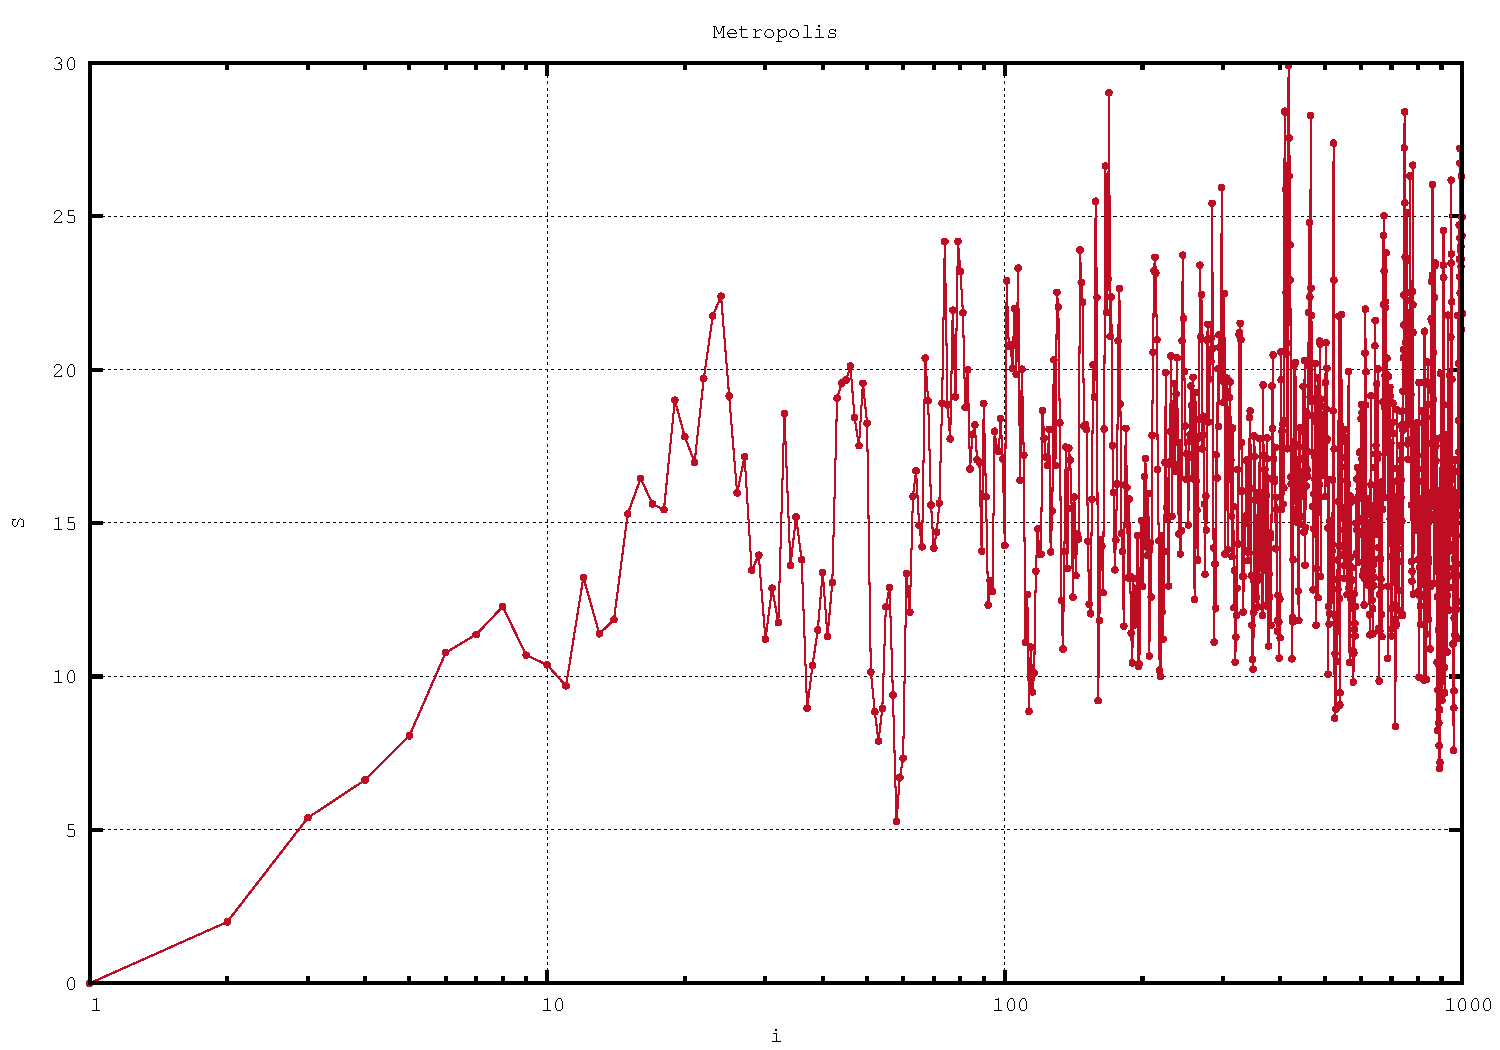
\includegraphics[width=\textwidth]{action1}
\caption{Cold Start}
\label{fig:action1}
\end{figure}
\begin{figure}[H]
\centering
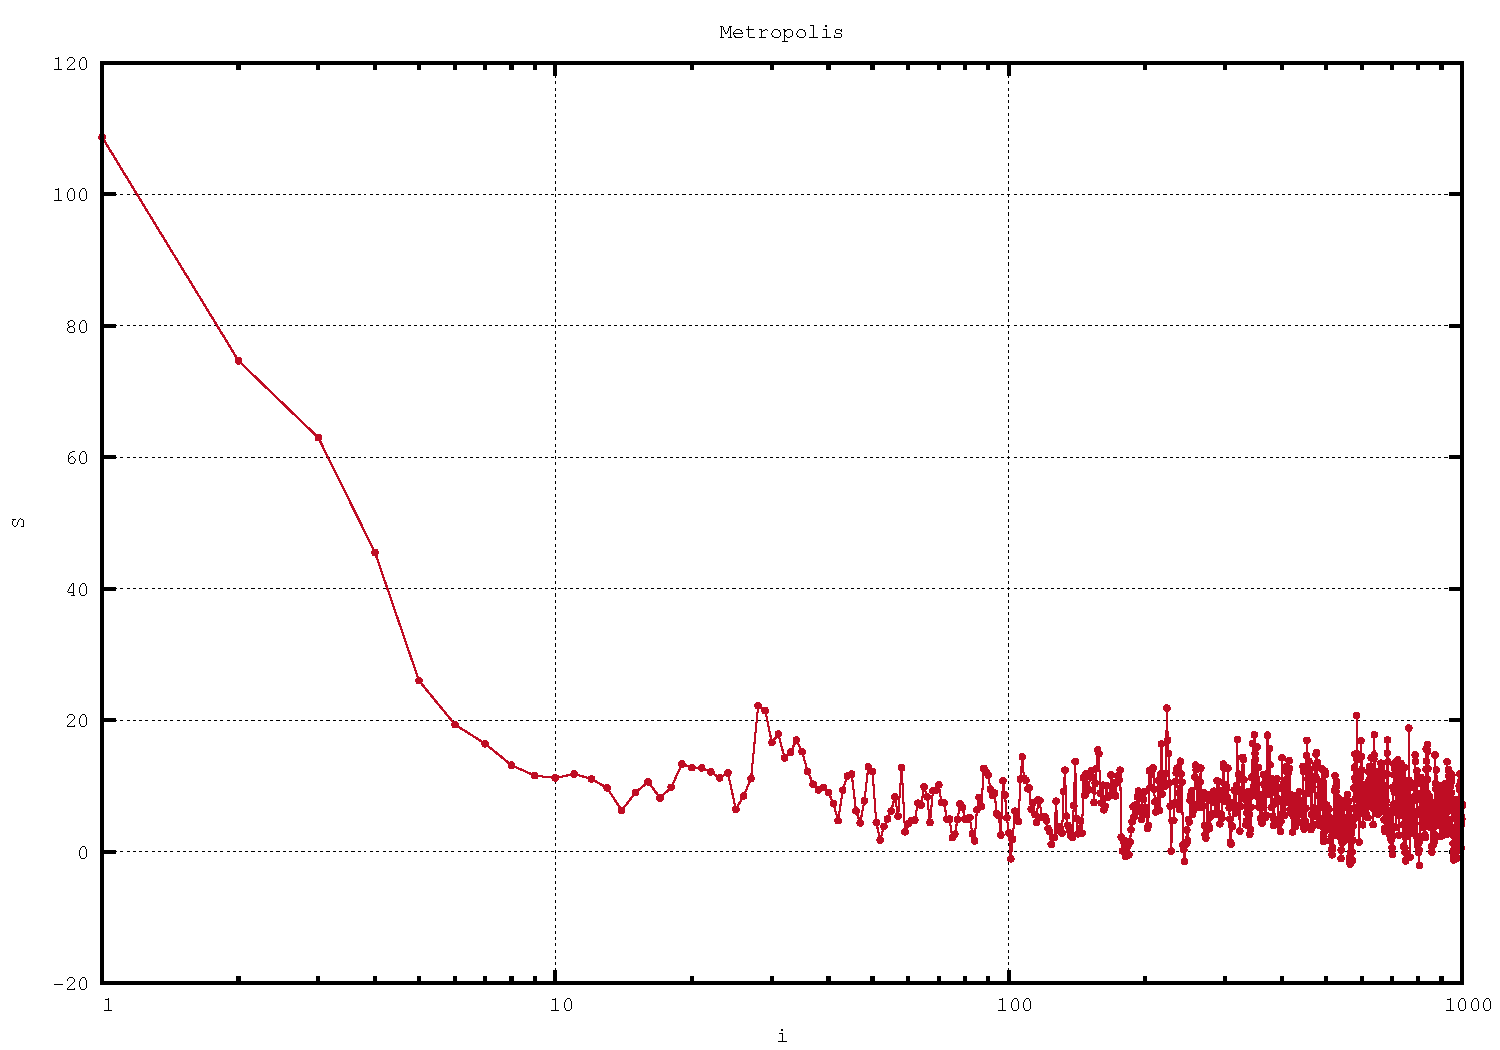
\includegraphics[width=\textwidth]{action2}
\caption{Hot Start}
\label{fig:action2}
\end{figure}

Per il calcolo dell'azione euclidea si usa la formula
$$S = a\displaystyle\sum\limits_{i=0}^{N-1} \mathcal{L}(x_{i},x_{i+1})$$
dove
$$\mathcal{L}(x_{i},x_{i+1}) = \frac{m}{2}\left(\frac{x_{i}-x_{i+1}}{a}\right)^{2}-\frac{1}{2}V(x_{i})-\frac{1}{2}V(x_{i+1})$$
Tuttavia, per calcolare $\Delta S = S'-S$ si può tenere presente il fatto che ad ogni estrazione solo una variabile di sistema viene modificata e quindi tutti i termini delle due sommatorie che non contengono quella variabile si elidono nella differenza. Pertanto si utilizza la formula ridotta
\begin{eqnarray*}
 \Delta S_i &=& a[\mathcal{L}(x_{i-1},x'_{i})+\mathcal{L}(x'_{i},x_{i+1})-\mathcal{L}(x_{i-1},x_{i})-\mathcal{L}(x_{i},x_{i+1})]\\
   &=& \tfrac{m}{a}[(x_{i}-x'_{i})(x_{i+1}+x_{i-1})+(x'^2_i-x^2_i)]+aV(x'_i)-aV(x_i)
\end{eqnarray*}

È facile verificare che l'algoritmo e i risultati possono essere resi indipendenti dal fattore di reticolo $a$ se si ridefiniscono propriamente i parametri del problema, il che è equivalente a porre $a=1$.
\newpage
\subsection{Autocorrelazione}

Si studia ora la correlazione tra configurazioni generate a step consecutivi dell'algoritmo per ottenere una stima del tempo di decorrelazione $\tau_d$ del sistema. Tale dipendenza fra elementi della catena viene anche denominata \textit{autocorrelazione}.

La formula per il correlatore di due stime dell'osservabile $O$ calcolate da stati estratti a istanti di tempo distanti $\tau$ è
$$R(\tau)=\frac{\langle O_iO_{i+\tau}\rangle-\langle O_i\rangle^2}{\langle O_i^2\rangle-\langle O_i\rangle^2}=\frac{\frac{1}{n-\tau}\sum\limits_{i=0}^{n-\tau}O_iO_{i+\tau}-\langle O_i\rangle^2}{\langle O_i^2\rangle-\langle O_i\rangle^2}\simeq e^{-\tfrac{\tau}{\tau_d}}$$

Il grafico dell'autocorrelazione $R(\tau)$ per l'osservabile $O(|l-k|)=\langle x_lx_k\rangle$ evidenzia la perdita esponenziale di correlazione nel segnale.
\begin{figure}[H]
\centering
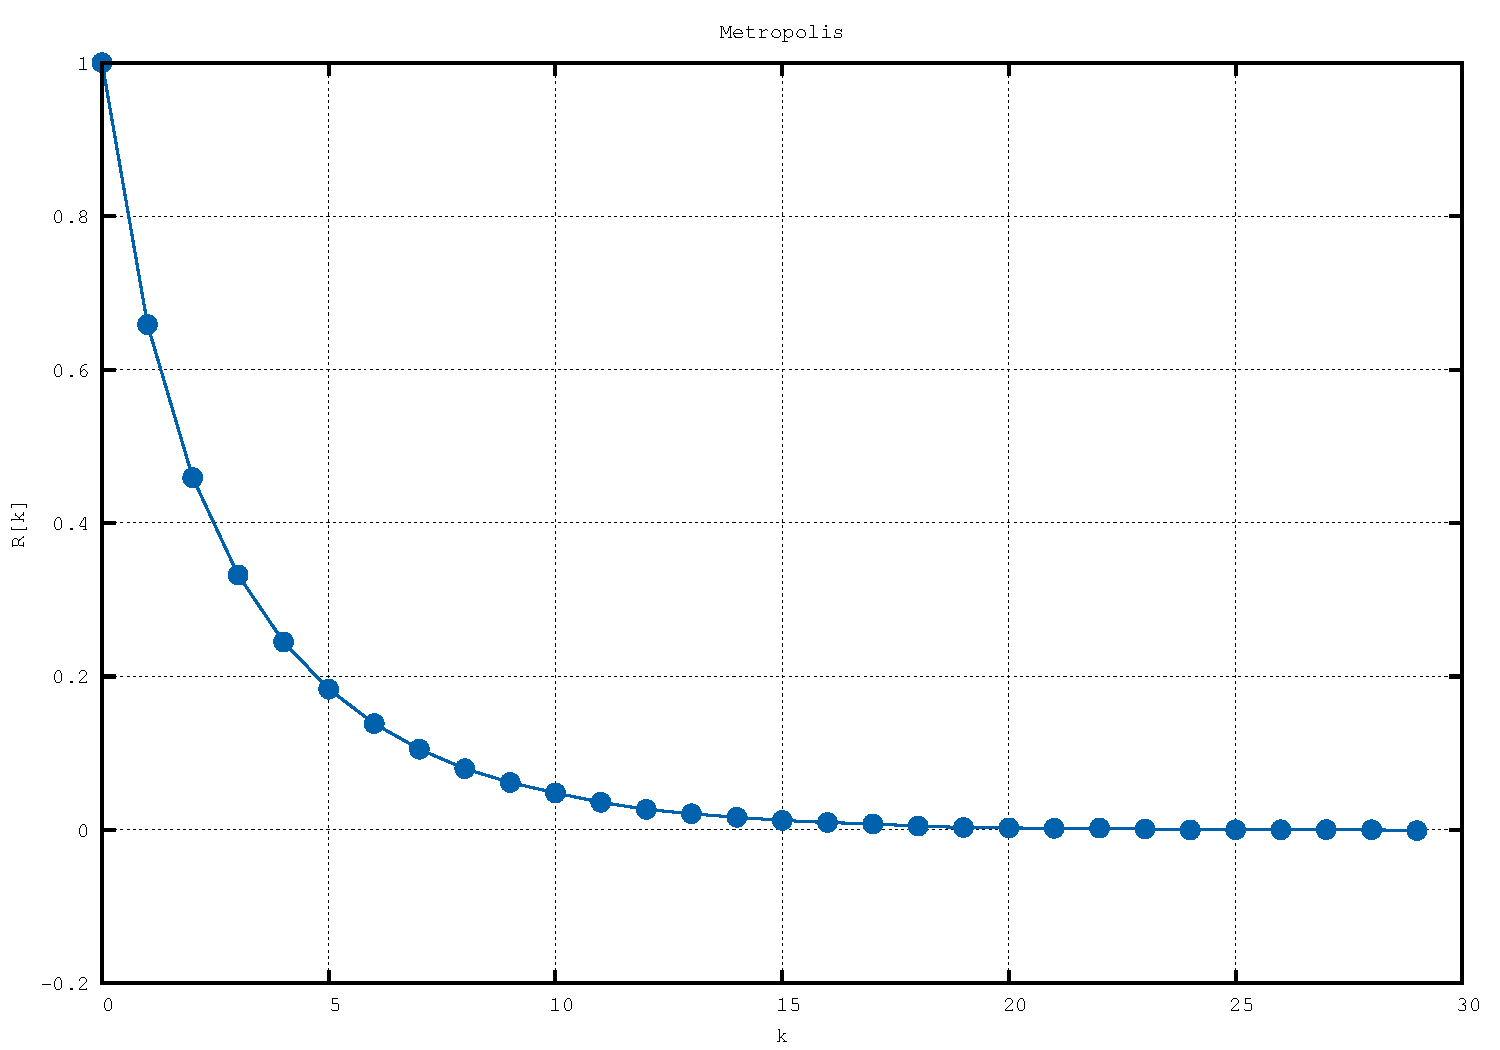
\includegraphics[width=\textwidth]{autocorrelation}
\caption{Autocorrelazione dell'osservabile $\langle x_lx_k\rangle$ per tutti i valori di $|l-k|$}
\label{fig:autocorrelation}
\end{figure}
Il tempo di decorrelazione $\tau_d$ è dell'ordine delle unità ($\sim3$) e quindi, per $\tau>5\tau_d\sim15$ il segnale può essere considerato praticamente scorrelato.
\newpage
\subsection{Funzioni di Correlazione}

Si calcola numericamente l'integrale $\int Dx \ x_lx_ke^{-S_E}$ applicando i metodi Monte Carlo e Metropolis in congiunzione. Affinchè le configurazioni utilizzate siano statisticamente indipendenti, si raggruppano i sample in $bin$ e si utilizza l'insieme delle medie su ogni $bin$ come sample di configurazioni per il calcolo MC. In questo modo, se la dimensione dei $bin$ è molto maggiore di $\tau_d$, la media sul $bin$ attenua considerevolmente gli effetti di correlazione e perciò il nuovo sample può essere considerato statisticamente unbiased.
\\

La media di un generico osservabile $O$ calcolata in questo modo è analiticamente uguale a quella calcolata per mezzo del sample completo di ogni elemento estratto. La varianza sui valori medi, tuttavia, differisce dalla varianza semplice di un termine proporzionale alla covarianza fra le variabili.

\begin{figure}[H]
\centering
\begin{tabular}{|c|c|c|}
\hline
$\Delta t$ & $C(\Delta t)$ & $Var(C(\Delta t))$\\
\hline
0 & 0.480083 & 0.001332\\
1 & 0.178045 & 0.000712\\
2 & 0.065869 & 0.000509\\
3 & 0.024213 & 0.000448\\
4 & 0.008814 & 0.000431\\
5 & 0.003284 & 0.000431\\
6 & 0.001328 & 0.000432\\
7 & 0.000660 & 0.000439\\
8 & 0.000205 & 0.000433\\
9 & -0.000037 & 0.000428\\
10 & 0.000073 & 0.000427\\
11 & 0.000157 & 0.000428\\
12 & 0.000096 & 0.000433\\
13 & -0.000041 & 0.000443\\
14 & -0.000131 & 0.000495\\
15 & -0.000091 & 0.000644\\

\hline
\end{tabular}
\quad
\begin{tabular}{|c|c|c|}
\hline
$\Delta t$ & $C(\Delta t)$ & $Var(C(\Delta t))$\\
\hline
16 & -0.000183 & 0.000845\\
17 & -0.000091 & 0.000644\\
18 & -0.000131 & 0.000495\\
19 & -0.000041 & 0.000443\\
20 & 0.000096 & 0.000433\\
21 & 0.000157 & 0.000428\\
22 & 0.000073 & 0.000427\\
23 & -0.000037 & 0.000428\\
24 & 0.000205 & 0.000433\\
25 & 0.000660 & 0.000439\\
26 & 0.001328 & 0.000432\\
27 & 0.003284 & 0.000431\\
28 & 0.008814 & 0.000431\\
29 & 0.024213 & 0.000448\\
30 & 0.065869 & 0.000509\\
31 & 0.178045 & 0.000712\\
\hline
\end{tabular}
\caption{Valori del correlatore delle coordinate in funzione della loro separazione nel reticolo temporale.}
\label{tab:correlation}
\end{figure}

\begin{figure}[H]
\centering
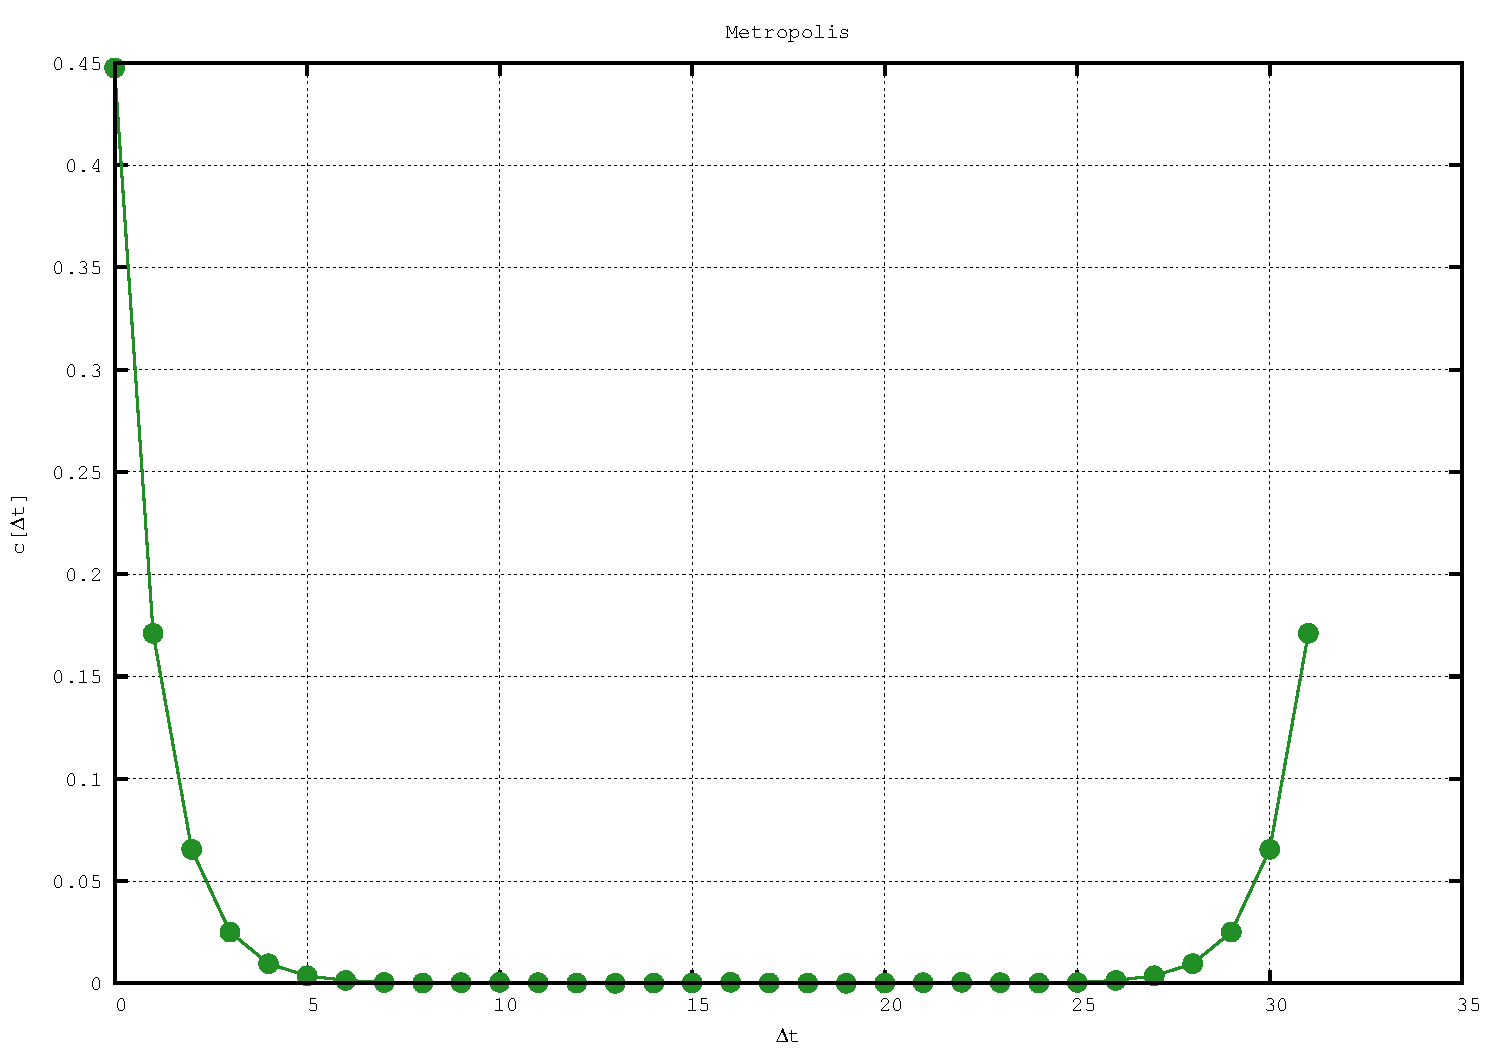
\includegraphics[width=\textwidth]{correlation}
\caption{L'andamento del correlatore delle coordinate è quello di un coseno iperbolico centrato in $|l-k|=\tfrac{N}{2}$. }
\label{fig:correlation}
\end{figure}
Sebbene il correlatore calcolato abbia un andamento complessivo in accordo con quello previsto dalla teoria, per valori di $\Delta t$ compresi fra $8$ e $24$ il segnale viene perso e prevale il rumore.

\subsection{Calcolo di Grandezze Quanto-Meccaniche Secondarie}

Come anticipato nell'introduzione sull'oscillatore armonico, è ora possibile ricavare stime di grandezze quanto-meccaniche secondarie direttamente dai valori delle funzioni di correlazione $C(\Delta t)=\langle x_tx_{t+\Delta t}\rangle$ del sistema.
Le varianze sui valori medi sono calcolate attraverso la tecnica \textit{cluster jackknife}.
\\

Sia $o_i$ la stima semplice dell'osservabile $O$ allo step $i$. La tecnica \textit{cluster jackknife} consiste nel ricavare le grandezze derivate $o^i$ (\textit{clusterization}), definite come $$o^i=\langle o\rangle+\frac{\langle o\rangle-o_i}{N_{bin}-1}$$ dove $N_{bin}$ indica il numero totale di $bin$. Nel caso in esame la grandezza $O$ è il correlatore calcolato nella sezione precedente ed è clusterizzato con $bin$ di ampiezza $100$ $(\gg\tau_d)$. Data una funzione $f=f(o)$, si definiscono $f^i=f(o^i)$ e $\langle f\rangle=f(\langle o\rangle)$. Si ottiene allora $$\sigma^2_f=\frac{N_{bin}-1}{N_{bin}}\sum\limits_i(f^i-\langle f\rangle)^2$$

Si ricavano dunque le formule per l'energia $\Delta E$ e l'elemento di matrice $W$. Per comodità di pone $\lambda\equiv N/2-\Delta t$ e si utilizza il seguente trucco per ricavare $\Delta E$ dalla formula per il correlatore $C$:
\begin{eqnarray*}
 \lefteqn{\frac{C(\Delta t-1)+C(\Delta t+1)}{2C(\Delta t)}=}\\
\\
   && =\frac{\tfrac{1}{2} (e^{a\Delta E(\lambda+1)}+e^{-a\Delta E(\lambda+1)})+\tfrac{1}{2} (e^{a\Delta E(\lambda-1)}+e^{-a\Delta E(\lambda-1)})}{2\tfrac{1}{2} (e^{a\Delta E\lambda}+e^{-a\Delta E\lambda})}=\\
\\
   && =\frac{(e^{a\Delta E}+e^{-a\Delta E})(e^{a\Delta E\lambda}+e^{-a\Delta E\lambda})}{2(e^{a\Delta E\lambda}+e^{-a\Delta E\lambda})}=\cosh(a\Delta E)
\end{eqnarray*}

$$\Rightarrow a\Delta E=\cosh^{-1}\left(\frac{C(\Delta t-1)+C(\Delta t+1)}{2C(\Delta t)}\right)$$
Trascurando il fattore $a$ e utilizzando i valori medi di $C$ calcolati su i $cluster$ si ottiene:
$$\Delta E = \cosh^{-1}\left(\frac{\langle C(\Delta t+1)\rangle+\langle C(\Delta t-1)\rangle}{2 \langle C(\Delta t)\rangle}\right)$$
$$W=\sqrt{\langle C(\Delta t)\rangle\frac{\exp\left(\Delta EN/2\right)}{2\cosh(\Delta E(N/2-\Delta t))}}$$
La migliore stima di $\Delta E$ e $W$ viene quindi calcolata come media sui valori dati dalle precedenti formule utilizzando i valori del correlatore per $0\le\Delta t\le6$.
\\

I valori utilizzati per i parametri del sistema sono $N=32$, $\hbar=1$, $a=1$, $\omega=1$, $m=1$, $\delta=3$ con un numero di sweep pari a $10^6$. I valori ottenuti sono distribuiti gaussianamente attorno ai valori medi che possono essere quindi ricavati dal fit di gaussiane agli istogrammi dei sample:
\begin{figure}[H]
\centering
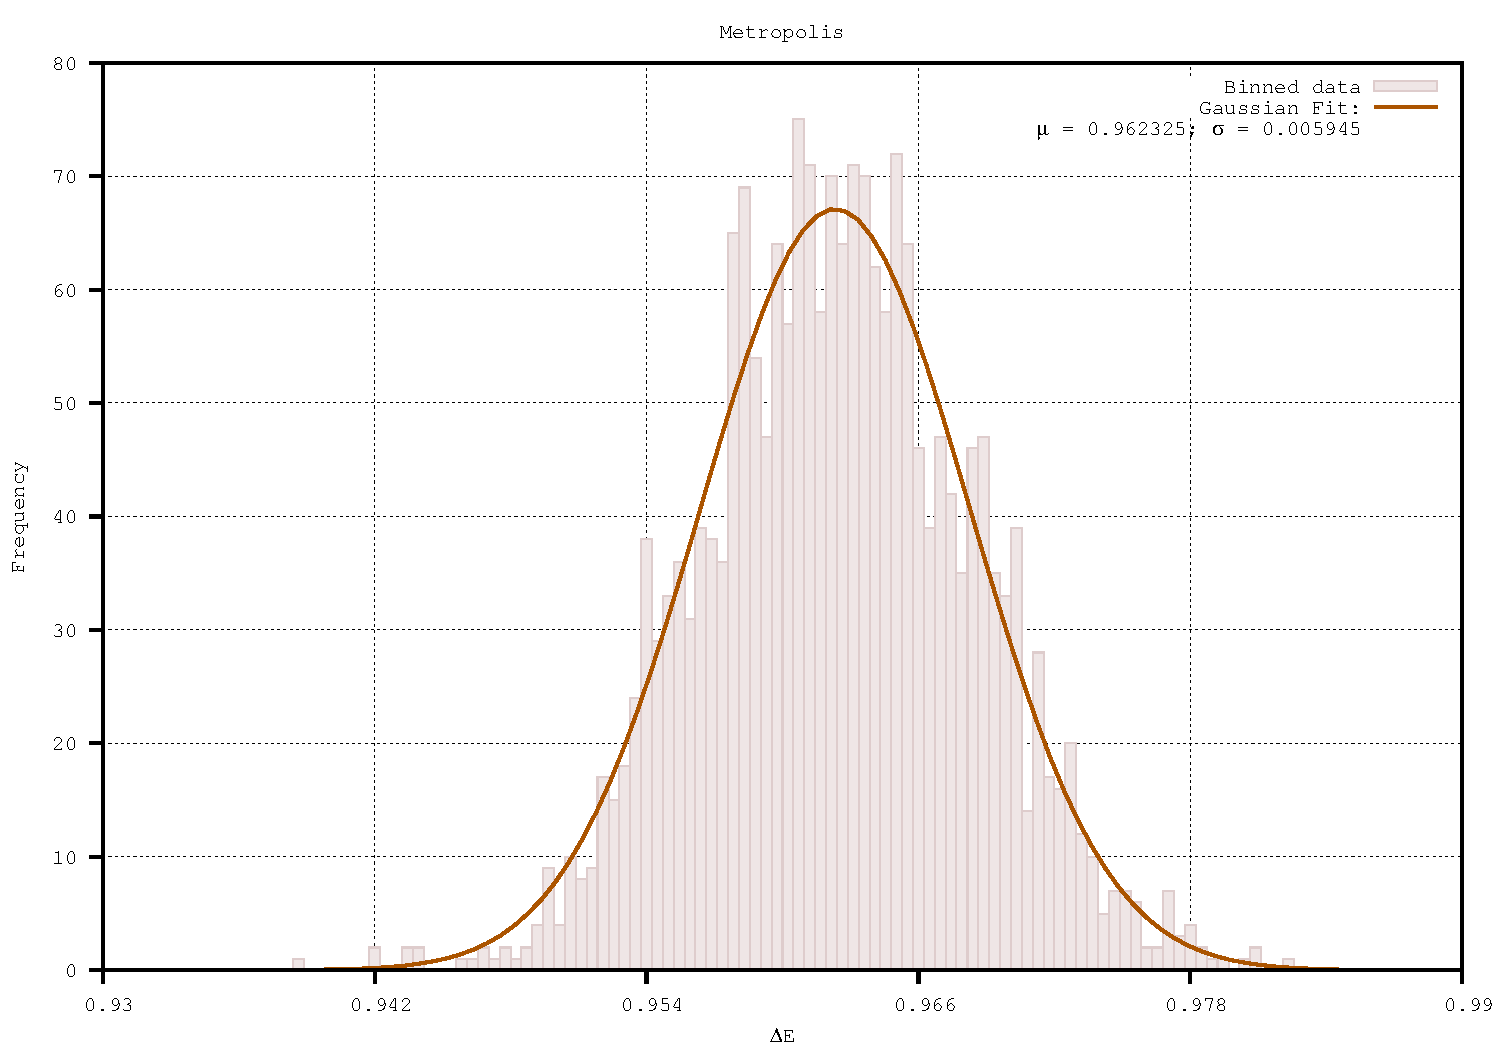
\includegraphics[width=0.65\textwidth]{histogram}
\caption{Distribuzione di $\Delta E$ a fissato numero di sweeps}
\label{fig:histogram}
\end{figure}
Risultati dei fit:
\begin{eqnarray*}
\Delta E&=&0.962325\pm0.005945\\
W&=&0.667925\pm0.007161
\end{eqnarray*}

Si nota inoltre che anche l'errore stimato dal \textit{cluster jackknife} è ditribuito gaussianamente intorno ad un valore molto vicino all'errore statistico ricavato dal fit.
\\

Si studia ora l'andamento della varianza $\sigma^2_{jackknife}$ in funzione del numero di $sweeps$.
\begin{figure}[H]
\centering
\begin{tabular}{|c|c|}
\hline
$N_{sweeps}$ & $\sigma^2_{jackknife}$\\
\hline
1000 & 2.087426e-02\\
2000 & 1.201255e-02\\
4000 & 6.999672e-03\\
8000 & 5.147464e-03\\
16000 & 2.081578e-03\\
32000 & 9.692904e-04\\
64000 & 5.851014e-04\\
128000 & 2.368376e-04\\
256000 & 1.377607e-04\\
512000 & 6.941350e-05\\
1024000 & 3.300726e-05\\
2048000 & 1.669044e-05\\
4096000 & 8.221103e-06\\
8192000 & 4.123789e-06\\
16384000 & 2.054391e-06\\
32768000 & 1.029125e-06\\
65392000 & 5.224967e-07\\
\hline
\end{tabular}
\label{tab:variance_tab}
\end{figure}
Rappresentando i dati ricavati dalle simulazioni in un grafico in scala bilogaritmica appare evidente che la varianza è inversamente proporzionale al numero di $sweeps$.
\begin{figure}[H]
\centering
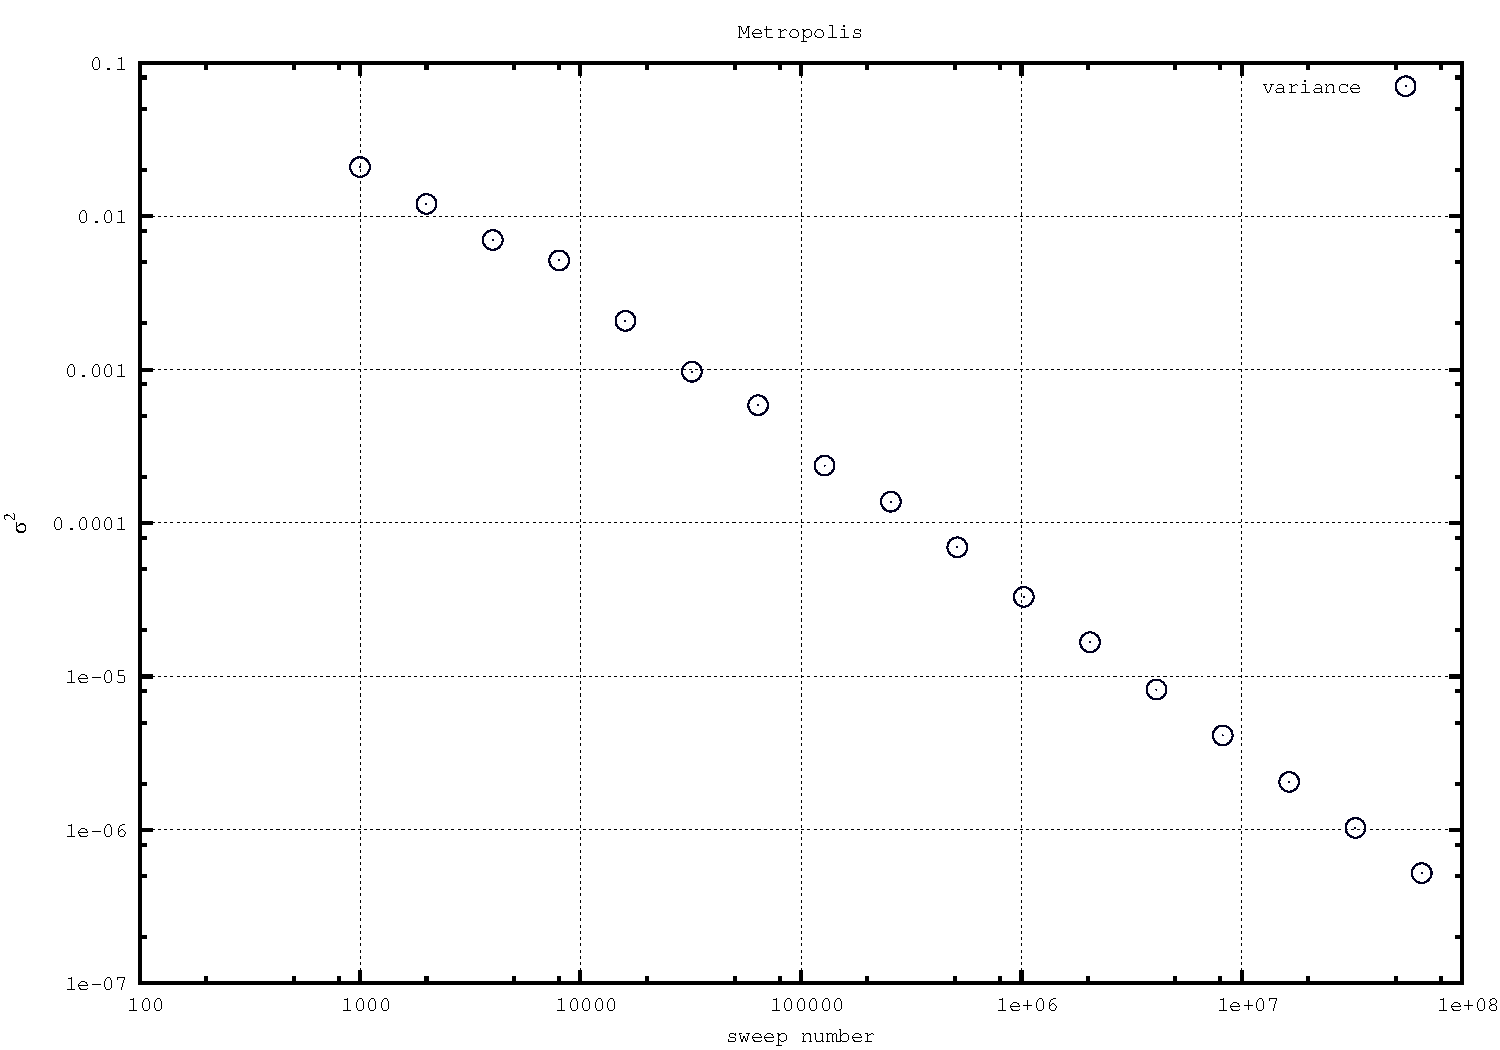
\includegraphics[width=\textwidth]{variance}
\caption{Varianza di $\Delta E$ in funzione del numero di sweeps}
\label{fig:variance}
\end{figure}
Interpolando linearmente il logaritmo dei dati sia sulle ascisse che sulle ordinate si ottiene infatti un coefficiente angolare $m=-0.976\sim-1$. Se ne deduce quindi che: 
$$\sigma\sim1/\sqrt{N_{sweeps}}$$

\chapter{\huge Metodo Runge-Kutta}

\textit{In analisi numerica i metodi Runge-Kutta sono una famiglia di metodi iterativi impliciti ed espliciti per la risuluzione approssimata di equazioni differenziali ordinarie (ODE). Il più comune di questi metodi è il cosidetto ``RK4'' o anche Runge-Kutta del quarto ordine.}
\\\\
Sia dato il problema di Cauchy
\begin{center}
$ \dot y = f(t, y), \quad y(t_0) = y_0.$
\end{center}
Si assume che il tempo sia discretizzato in istanti $t_n$ equidistanziati di un intervallo $h$.\\
Il metodo RK4 per questo problema è allora dato dalle seguenti equazioni:
\begin{eqnarray*}
y_{n+1} &=& y_n + \tfrac{1}{6} \left(k_1 + 2k_2 + 2k_3 + k_4 \right)\\
t_{n+1} &=& t_n + h
\end{eqnarray*}
dove $y_{n+1}$ è l'approssimazione RK4 di $y(t_{n+1})$, e
\begin{eqnarray*}
k_1 &=& hf(t_n, y_n),\\
k_2 &=& hf(t_n + \tfrac{1}{2}h , y_n + \tfrac{1}{2} k_1),\\
k_3 &=& hf(t_n + \tfrac{1}{2}h , y_n + \tfrac{1}{2} k_2),\\
k_4 &=& hf(t_n + h , y_n + k_3).
\end{eqnarray*}
Il valore della funzione $y$ all'istante $t_{n+1}$ è uguale quindi al suo valore all'istante $t_n$ incrementato della media ponderata di quattro incrementi $k$, dove ogni incremento è il prodotto della dimensione dell'intervallo $h$ ed una stimata pendenza specificata dalla funzione $f$.
\begin{itemize}
\item $k_1$ è l'incremento basato sulla pendenza di $f$ all'estremo sinistro dell'intervallo, calcolato in $y_n$ (metodo di Eulero);
\item $k_2$ è l'incremento basato sulla pendenza nel punto medio dell'intervallo, calcolato in $y_n+\frac{1}{2}k_1$;
\item $k_3$ è ancora l'incremento basato sulla pendenza nel punto medio, calcolato però in $y_n+\frac{1}{2}k_2$;
\item $k_4$ è l'ncremento basato sulla pendenza all'estremo destro dell'intervallo, calcolato in $y_n+k_3$.
\end{itemize}
Si nota dalla formula per $y_{n+1}$ che peso maggiore viene assegnato all'incremento al centro dell'intervallo. Inoltre, se $f=f(t)$ cioè non dipende da $y$, il metodo RK4 si riduce alla regola di integrazione di Simpson.

RK4 è un metodo del quarto ordine e quindi l'errore ad ogni step è dell'ordine di $h^5$, mentre l'errore totale accumulato è dell'ordine di $h^4$.

\section{Il Pendolo Caotico}
Il sistema che si intende simulare è quello dell'oscillatore caotico forzato di equazione
\begin{center}
$\ddot{\theta} = \underbrace{\frac{g}{R}}_1 \sin(\theta)-\underbrace{\frac{k}{m}}_q \dot{\theta}+\underbrace{\frac{f}{mR}}_b \cos(\omega t)$.
\end{center}
È possibile rielaborare l'equazione precedente in un sistema di equazioni differenziali del primo ordine come di seguito
$$\begin{system}
\dot\theta&=\phi \\[1ex] \dot\phi&=\sin(\theta)-q\phi+b\cos(\omega t)
\end{system}$$
ed applicare ora la formula del metodo RK4 ad entrambe le equazioni.

Rappresentando la traiettoria del sistema nello spazio delle fasi si ottiene
\begin{figure}[h!]
\centering
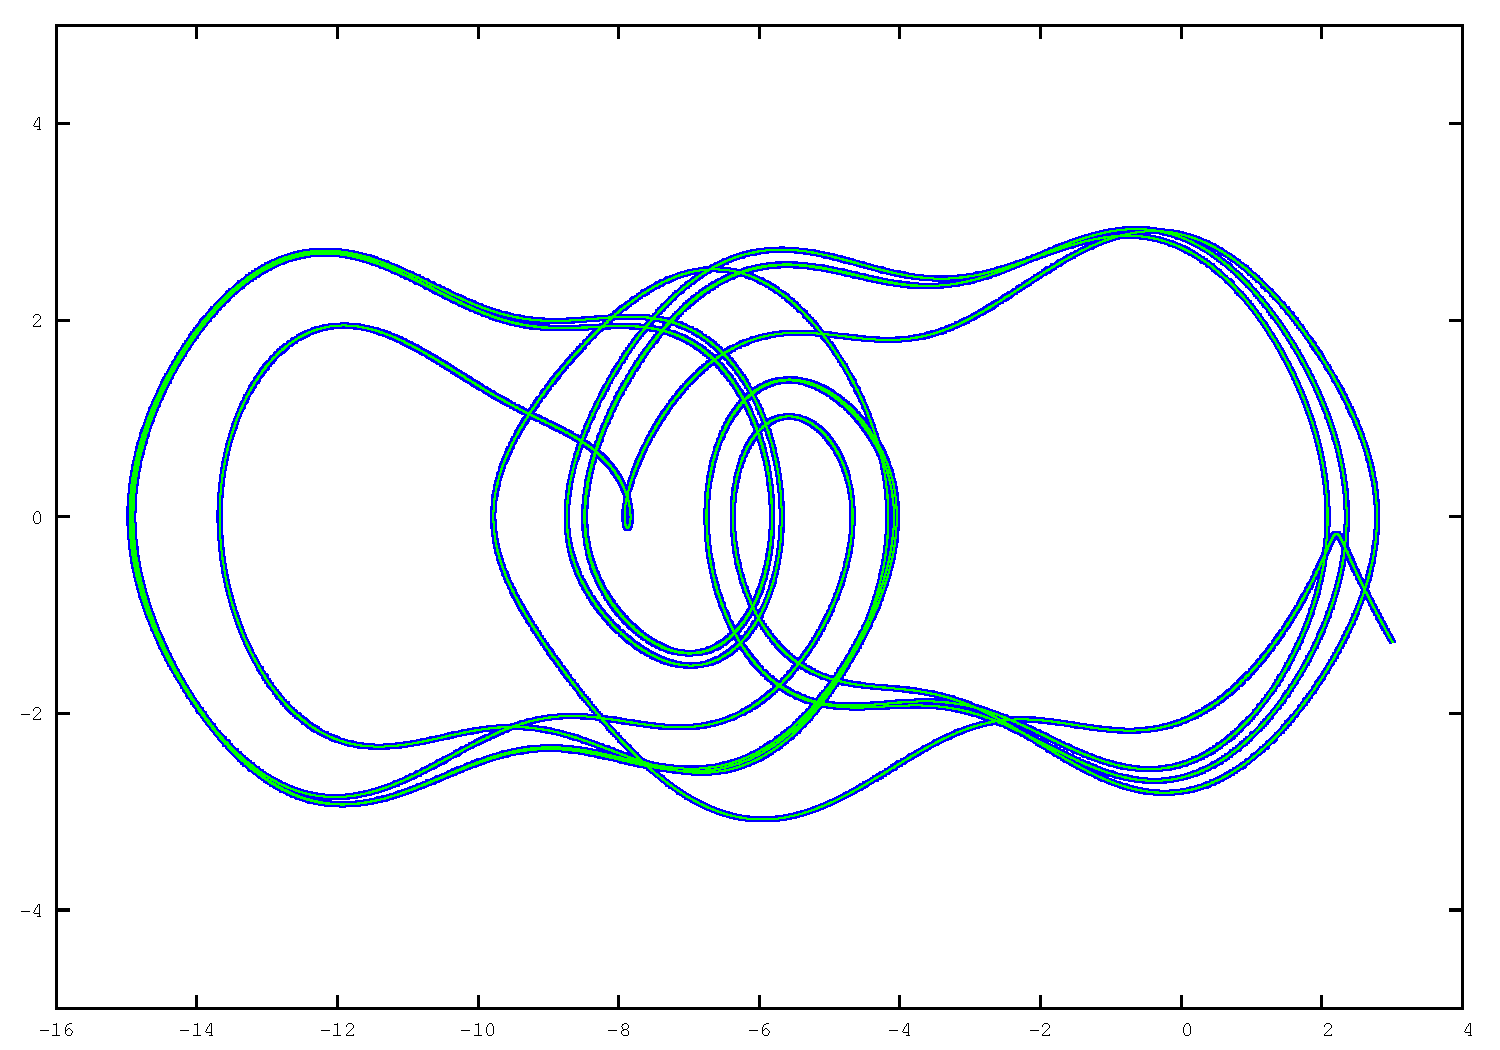
\includegraphics[width=\textwidth]{chaotic}
\caption{Traiettoria dell'oscillatore per $q = 0.3$, $b = 1.4$, $\omega = 0.6667$}
\label{fig:chaotic}
\end{figure}

\section{Oscillatore di Van Der Pol}
Analogamente al caso dell'oscillatore caotico, si applica il metodo RK4 all'equazione del pendolo di Van Der Pol, che in questo caso è
\begin{center}
$\frac{d^2x}{dt^2}-\mu(1-x^2)\frac{dx}{dt}+x= 0$
\end{center}
dove $\mu$ rappresenta l'intensità dello smorzamento. Il sistema associato è
$$\begin{system}
\dot x&= y\\[1ex] \dot y&=\mu(1-x^2)\frac{dx}{dt}-x
\end{system}$$

\begin{figure}[h!]
\centering
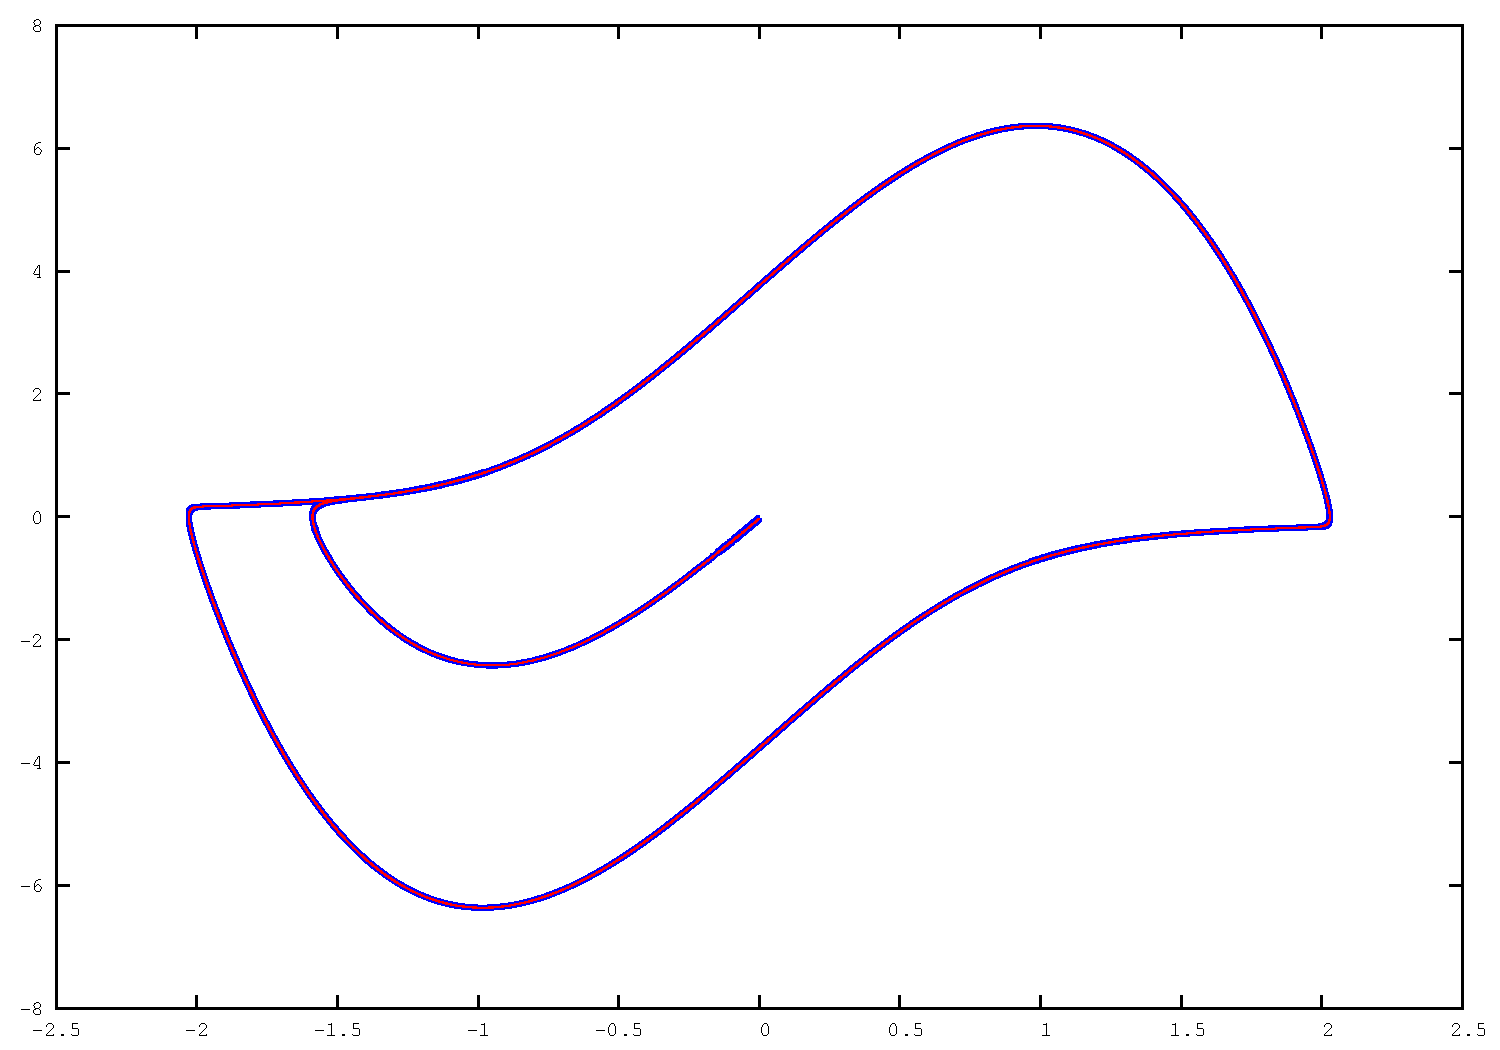
\includegraphics[width=\textwidth]{vanderpol}
\caption{Traiettoria dell'oscillatore per $\mu = 4$}
\label{fig:vanderpol}
\end{figure}
Anche in questo caso si può osservare un ciclo limite nello spazio delle fasi del sistema, ovvero una traiettoria chiusa verso la quale il sistema è portato ad evolvere.

\section{Attrattore di Lorenz}
\begin{figure}[h!]
\centering
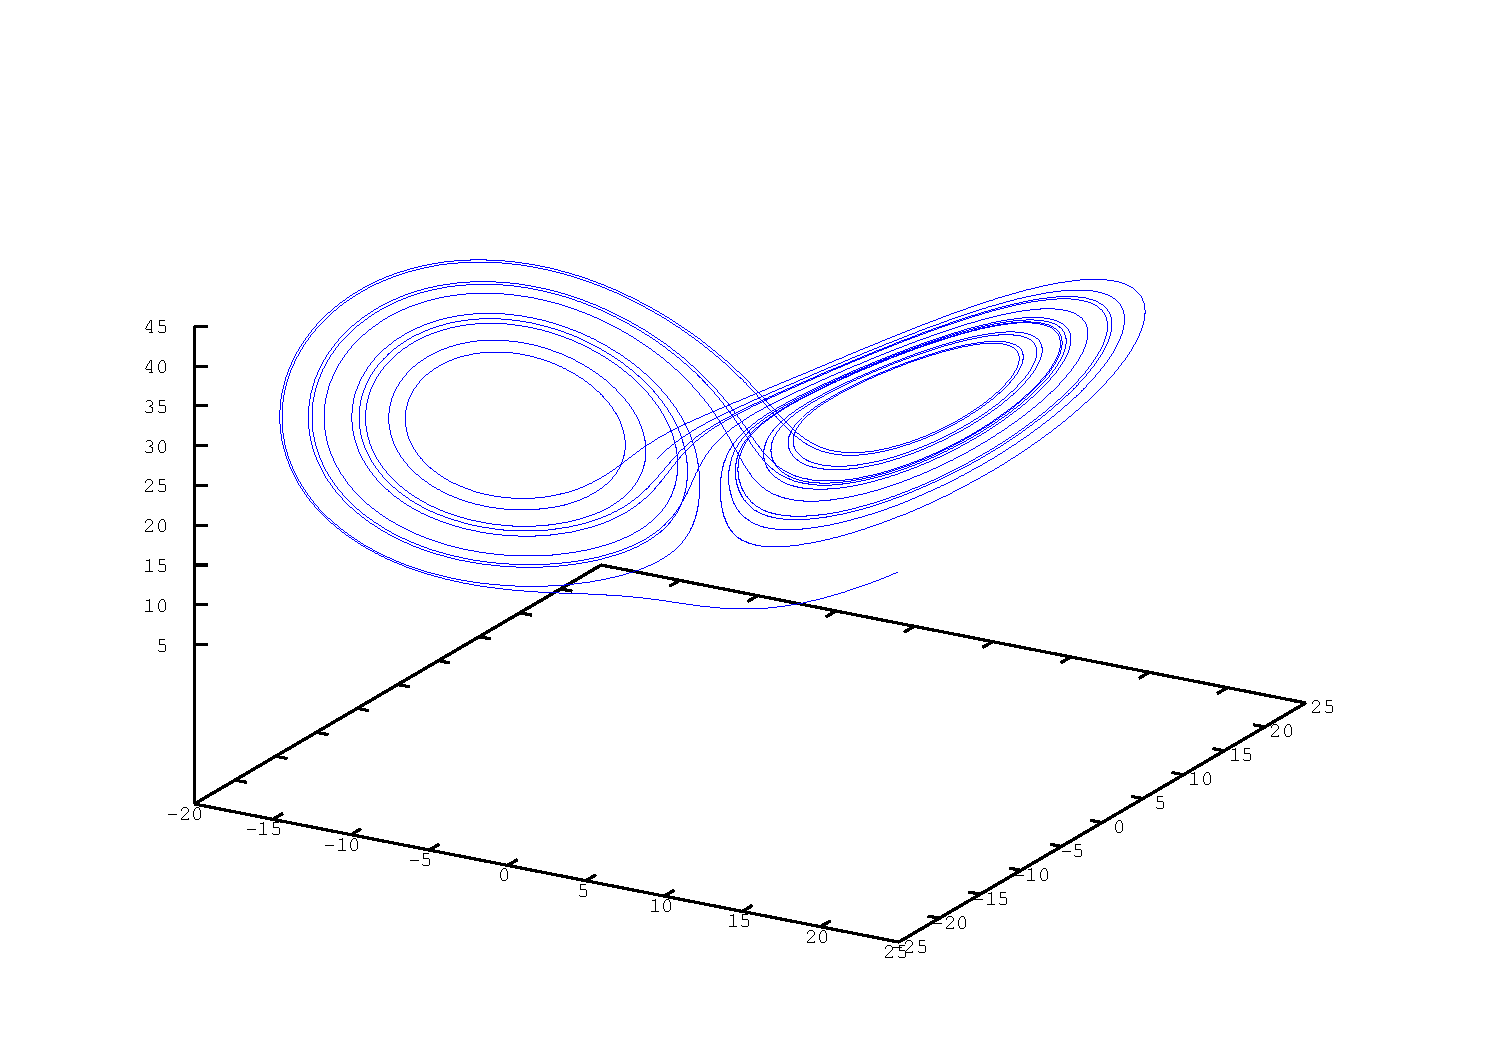
\includegraphics[width=0.33\textwidth]{lorenz0}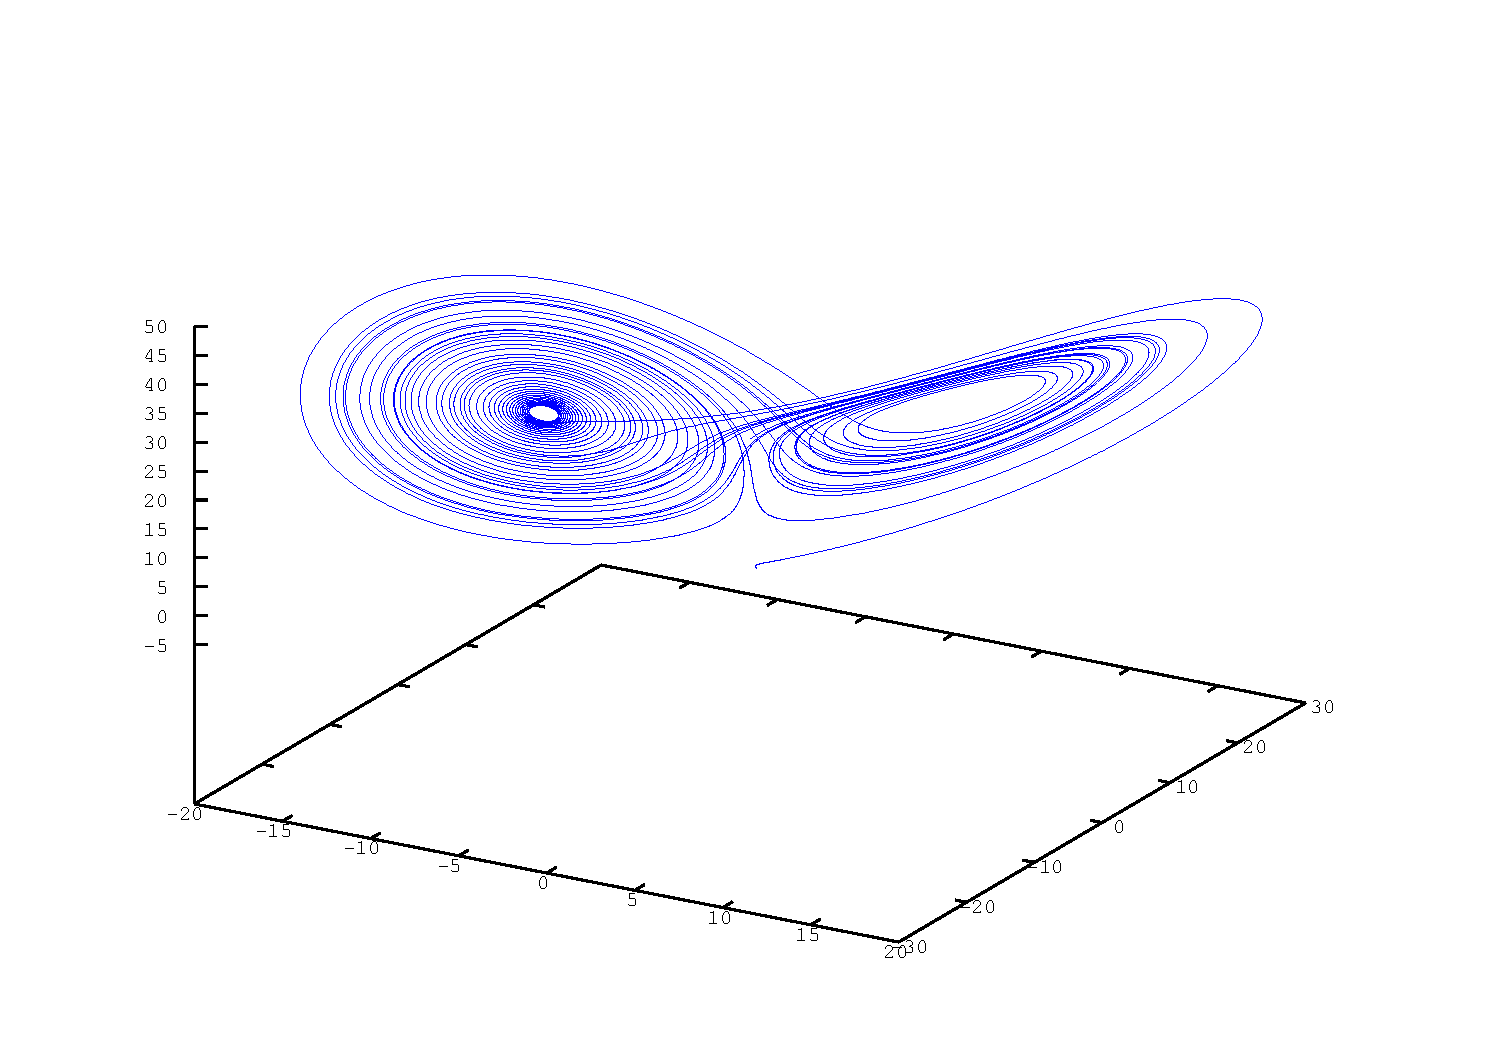
\includegraphics[width=0.33\textwidth]{lorenz1}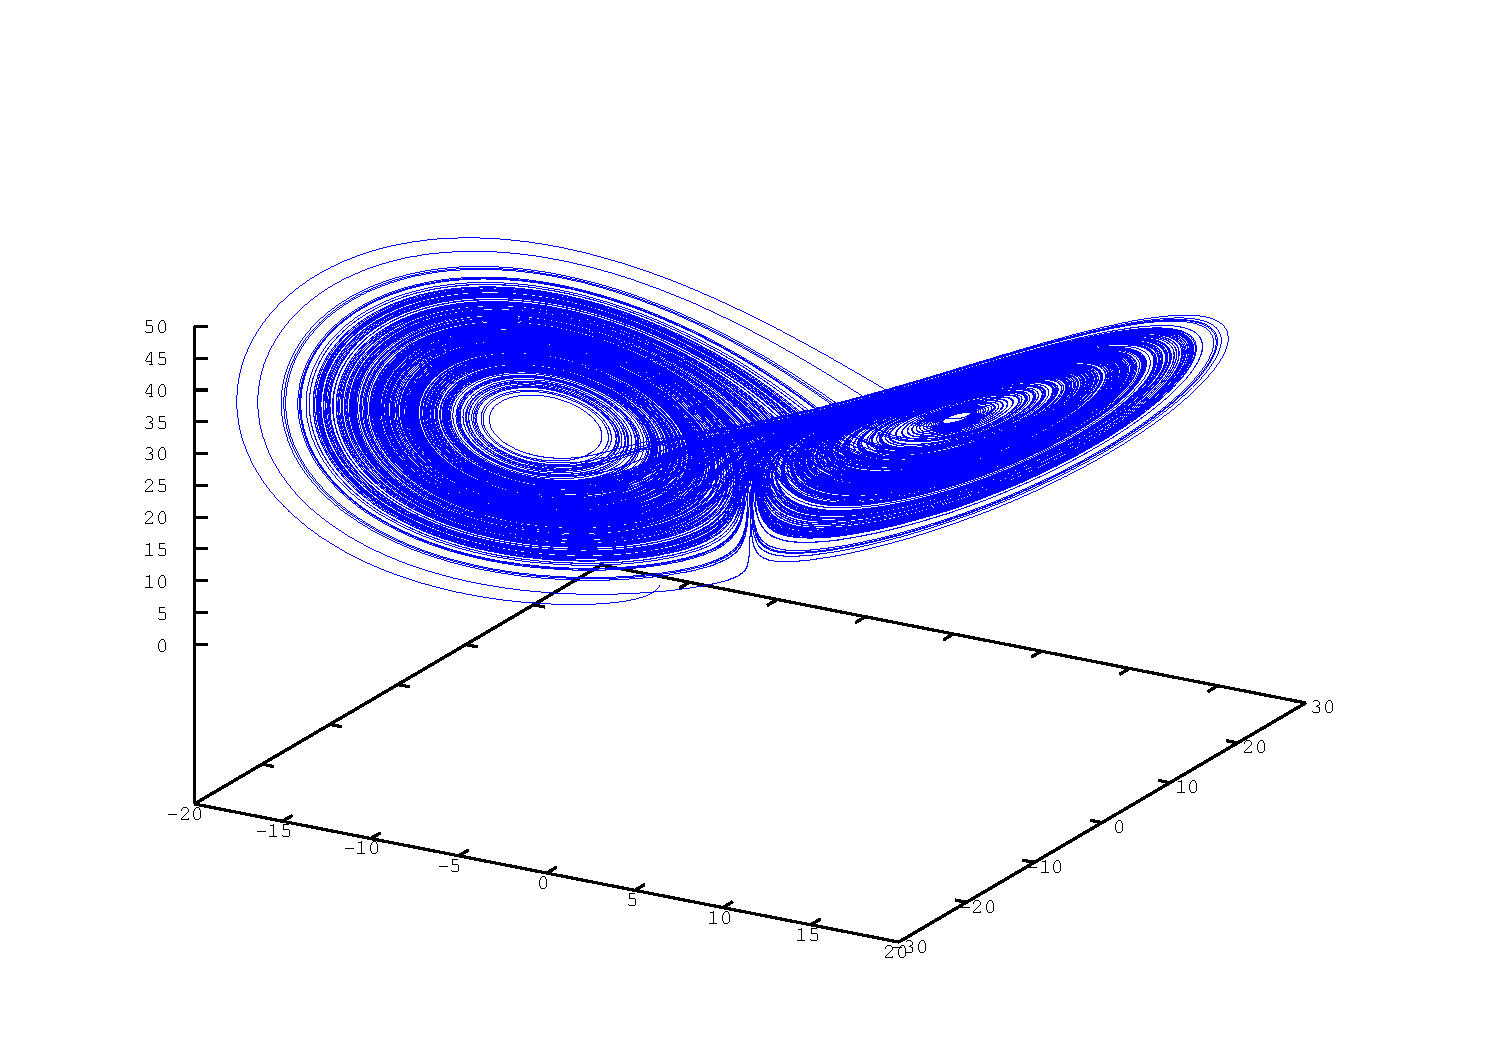
\includegraphics[width=0.33\textwidth]{lorenz2}
\caption{Sistema di Lorenz in tre dimensioni}
\label{fig:lorenz}
\end{figure}


\chapter{\huge Metodo implicito}

\textit{Per sistemi di equazioni alle derivate parziali (PDE) esistono altri metodi oltre a quelli RK. In questa sezione si illustra e implementa il cosidetto metodo implicito per risolvere equazioni agli operatori lineari.}

\begin{figure}[H]
\centering
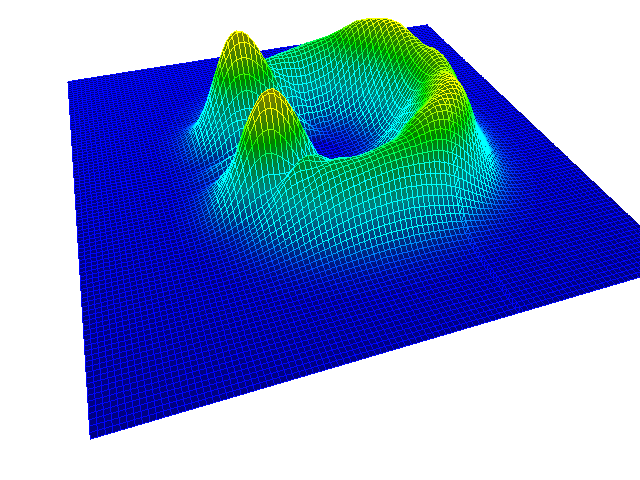
\includegraphics[width=\textwidth]{schrodinger}
\caption{Scattering di un pacchetto gaussiano con una buca di potenziale}
\label{fig:schrodinger}
\end{figure}

\section{Equazione di Schr\"{o}dinger}

L'equazione che si intende risolvere è l'equazione di Schr\"odinger dipendente dal tempo
$$i\hbar\frac{\partial}{\partial t} \psi(x,\,t) = -\frac{\hbar^2}{2m}\nabla^2\psi(x,\,t) + V(x)\psi(x,\,t)$$
A tal fine si discretizza lo spazio in modo tale che $x=na$ con $n=0,...,N-1$ ed $a$ passo del reticolo spaziale. $\psi(x,\,t)$ diventa quindi un vettore di valori complessi $\psi_n(t)$. Si pongono inoltre condizioni di periodicità al contorno di modo che $\psi_N \equiv \psi_0$.

Con questa dicretizzazione si sostituisce
$$\nabla^2\psi(x) \rightarrow \frac{\psi_{n+1}+\psi_{n-1}-2\psi_n}{a^2} $$
pertanto l'equazione diventa
$$i\hbar\frac{\partial}{\partial t} \psi_n = -\frac{\hbar^2}{2m}\frac{\psi_{n+1}+\psi_{n-1}-2\psi_n}{a^2} + V_n\psi_n = \sum\limits_{n}A_{n,m}\psi_m$$
La soluzione dell'equazione è la funzione esponenziale
$$\psi(t)=\exp(-\frac{i}{\hbar}At)\psi(0)$$
dove $U(t) = \exp(-\frac{i}{\hbar}At)$ rappresenta l'evolutore temporale del sistema. Sviluppando ora $U(t)$ intorno all'unita per $t\rightarrow 0$ e trascurando gli ordini superiori in $t$ si ottiene la formula approssimata
$$\psi(t_0+t)=\psi(t_0)-\frac{i}{\hbar}At\psi(t_0)$$
Questa prima approssimazione tuttavia porta all'insorgere di numerosi problemi dovuti al fatto che l'iterazione del precedente passaggio non rispetta la condizione di unitarietà dell'operatore evolutore temporale. Bisogna quindi ricorrere ad una strategia più astuta.

Il \textbf{metodo implicito} consiste nell'approssimare l'operatore esatto $U(t)$ attraverso la formula
$$\psi(t+dt)=(1+\frac{i}{2\hbar}Adt)^{-1}(1-\frac{i}{2\hbar}Adt)\psi(t)$$
Utilizzando il fatto che $A$ è Hermitiano, è facile dimostrare che l'operatore della precedente formula è unitario proprio come $U(t)$.
Per implementare questo algoritmo iterativo è necessario risolvere ad ogni step il sistema lineare
$$(1+\frac{i}{2\hbar}Adt)\psi(t+dt)=(1-\frac{i}{2\hbar}Adt)\psi(t)$$

Infine si moltiplicano entrambi i membri dell'equazione per l'aggiunto dell'operatore a primo membro, in modo tale da ottenere
$$(1+\frac{1}{4\hbar^2}A^2dt^2)\psi(t+dt)=(1-\frac{i}{2\hbar}Adt)^2\psi(t)$$
dove ora $(1+\frac{1}{4\hbar^2}A^2dt^2)$ è Hermitiano e si può quindi risolvere rispetto a $\psi(t+dt)$ utilizzando il \textit{Conjugate Residual Method}.\\

L'idea che sta alla base di questo metodo è che se in un intervallo di tempo $dt$ la funzione $\psi(t)$ evolve in $\psi(t+dt)$, allora facendo evolvere $\psi(t)$ in avanti nel tempo per $\frac{dt}{2}$ e $\psi(t+dt)$ indietro nel tempo sempre di $\frac{dt}{2}$ le due funzioni dovranno coincidere.



\begin{thebibliography}{9}
\addcontentsline{toc}{chapter}{Bibliografia}
\bibitem{uno} M. Abramowitz, I. A. Stegun. ``§25.4, Integration'', \textit{Handbook of Mathematical Functions (with Formulas, Graphs, and Mathematical Tables)}, 1972
\bibitem{due} I. Beichl, F. Sullivan. \textit{Computing in Science and Engineering}, 2000
\bibitem{tre} M. Hjorth-Jensen. ``§9, Random walks and the Metropolis algorithm'', \textit{Computational Physics}, 2009
\bibitem{quattro} Y. Saad. \textit{Iterative Methods for Sparse Linear Systems}, 2003
\bibitem{cinque} C. Rebbi. \textit{Lecture Notes on Advanced Computing in Physics}, 1996
\bibitem{sei} S. Weinzierl. \textit{Introduction to Monte Carlo methods}, 2000
\end{thebibliography} 

\end{document}
